The appendices give the proofs and numerical details for the paper. In the Gaussian example, distribution error depends on scale, while particle error also depends on angle. The nonlinear example shows the same difference when the distribution changes shape. The general proof shows how the acceleration condition improves distribution accuracy in both examples. The table below gives the location of each result.

\begin{center}
\begin{tabular}{p{0.70\linewidth}l}
\toprule
Main claim or comparison & Support\\
\midrule
Finite-time $W_2$ bound and its coupling & Appendix~\ref{app:general}\\
Minimum action and the gradient-field consequence & Appendix~\ref{app:projection}\\
Gaussian distribution and particle errors & Appendix~\ref{app:fixed-gaussian}\\
Nonlinear rates, coefficient error, and extensions & Appendix~\ref{app:nonlinear}\\
Residual acceleration bound & Appendix~\ref{app:robustness}\\
Local converse and terminal cancellation & Appendix~\ref{app:local}\\
Solver dependence and equal NFE & Appendix~\ref{app:solver}\\
Mean, second-moment, and action restrictions & Appendix~\ref{app:obstruction}\\
Scaled rotated Gaussian coupling & Appendix~\ref{app:fm}\\
Weak expansion and regular displacement interpolation & Appendices~\ref{app:weak}, \ref{app:displacement}\\
Arbitrarily small action cost on one grid & Appendix~\ref{app:schedules}\\
Population calculations and refinement results & Appendix~\ref{app:numerics}\\
\bottomrule
\end{tabular}
\end{center}

For a map $F$, the pushforward $F_\#\mu$ is the distribution of $F(X)$ when $X\sim\mu$. We write $\mathcal P_2(\R^d)$ for probability measures with finite second moment, and define the root mean squared size of a vector field $w$ by
\[
 \|w\|_{L^2(p)}=\left(\int \|w(x)\|^2p(\dd x)\right)^{1/2}.
\]
For a random vector $Z$, $\|Z\|_{L^2}$ is its root mean squared norm. Table~\ref{tab:notation} lists the main symbols.

\begin{table}[ht]
\centering
\caption{Notation used in the proofs. Matrices and coefficients specific to an example are defined with that example.}
\label{tab:notation}
\begin{tabular}{lp{0.73\linewidth}}
\toprule
Symbol & Meaning\\
\midrule
$p_t$, $\widehat p_k$ & Exact distribution at time $t$ and Euler distribution at node $k$\\
$u_t$, $r_t$ & Velocity field and a correction added to that field\\
$\acc_t$, $\jerk_t$ & Second and third time derivatives along an exact particle\\
$T$, $h_k$, $H$ & Final time, step length, and largest step length\\
$W_2$ & Distribution distance from the best root mean squared pairing\\
$\cA_T$ & Kinetic action over the time interval $[0,T]$\\
$F_{s,t}$ & Exact particle flow from time $s$ to time $t$\\
$\Psi_t^\tau$ & Auxiliary acceleration flow with physical time $t$ held fixed\\
$L$, $L_a$ & Common spatial Lipschitz bounds for velocity and acceleration\\
$C_a$, $C_j$ & Uniform $L^2(p_t)$ bounds for acceleration and its material derivative\\
$\Sigma_0$, $\Omega$ & Initial Gaussian covariance and its weighted rotation matrix\\
$C_0$, $K_t$ & Gaussian covariance root and skew matrix in the rotation representation\\
$C_{w,2}$, $C_w$ & $L^2$ bound for $w_t$ and constant in the residual bound\\
$\alpha$, $\beta$, $\beta_a$ & Nonlinear radial rate, rotation rate, and tangential acceleration coefficient\\
$\mathcal C_i$, $\Theta_1$ & Leading radius-error and angle-error coefficient functions\\
$\mathcal T$, $G$, $d_{\rm aff}$ & Affine map, its matrix, and its shift\\
$R(t,r)$, $R_{i,k}(r)$ & Exact and numerical radii from starting radius $r$\\
\bottomrule
\end{tabular}
\end{table}
\FloatBarrier

\section{Fixed Gaussian correction and recursive errors}
\label{app:fixed-gaussian}

The Gaussian result also holds when the mean moves at constant velocity and the covariance is any positive definite matrix in even dimension. Assume $T,a>0$ and $\Sigma_0=C_0C_0^\top$, with $J^\top=-J$, $J^\top J=I$, and $\Omega=C_0JC_0^{-1}$. For $m_t=m_0+t\xi$, the fields $v_0(t,x)=\xi+a(x-m_t)$ and $v_1(t,x)=\xi+a(I+\Omega)(x-m_t)$ both generate $p_t=\mathcal N(m_t,e^{2at}\Sigma_0)$. These parameters stay fixed as the grid changes. The base field $v_0$ minimizes action among finite-action fields satisfying the same weak continuity equation. The correction increases action by
\[
 \cA_T(v_1)-\cA_T(v_0)=a^2\tr(\Sigma_0)\frac{e^{2aT}-1}{2a}>0.
\]
Euler reproduces $m_t$ exactly and has covariance $q_{i,k}\Sigma_0$, where
\[
 q_{0,k}=\prod_{j<k}(1+ah_j)^2,\qquad
 q_{1,k}=\prod_{j<k}(1+2ah_j+2a^2h_j^2).
\]
Euler's distribution error is $\sqrt{\tr(\Sigma_0)}[e^{at_k}-\sqrt{q_{i,k}}]$. The corrected error is positive and strictly smaller for every $k\ge1$. Equations~\eqref{eq:base-order}--\eqref{eq:particle-order} hold with $C_\Sigma=\sqrt{\tr(\Sigma_0)}e^{aT}$. Setting $m_0=\xi=0$ and $\Sigma_0=I_2$ gives Theorem~\ref{thm:fixed-gaussian}.

Write
\[
 I_a(T)=\int_0^T e^{2at}\dd t=\frac{e^{2aT}-1}{2a}.
\]
Subtracting the mean and applying the inverse covariance factor gives a Gaussian source with identity covariance. These coordinates are called whitened coordinates. Each corrected Euler step changes scale and angle, but rotation leaves the Gaussian distribution unchanged. Distribution error therefore depends only on scale. Particles from the same starting point also have an angle error. The scale error has a positive second-order coefficient, while the angle error has a positive first-order coefficient.

The correction belongs to the Gaussian family of \citet[Proposition~5.5]{lim2025hidden}. For a single Gaussian with $\Sigma_t=e^{2at}C_0C_0^\top$, the skew matrix $K_t=b e^{-2at}C_0^{-\top}JC_0^{-1}$ gives $\Sigma_tK_t(x-m_t)=b\Omega(x-m_t)$. This form lets us calculate kinetic action and Euler error over the full time interval.

\begin{proof}[Proof of Theorem~\ref{thm:fixed-gaussian} and its Gaussian extension]
\label{proof:fixed-gaussian}
\textbf{Common path and action.}\quad
The assumptions on $J$ imply $J^2=-I$. Direct matrix multiplication verifies
\[
 \Omega\Sigma_t+\Sigma_t\Omega^\top=0,\qquad
 \Omega\Sigma_t\Omega^\top=\Sigma_t,\qquad \Sigma_t=e^{2at}\Sigma_0.
\]
The centered flows $e^{at}I$ and $e^{at}C_0e^{atJ}C_0^{-1}$ both give covariance $\Sigma_t$ and mean $m_t$. Both flows are global and affine, so the distributions remain Gaussian. Equal means and covariances therefore give the same distribution at every intermediate time.

For $Y\sim\mathcal N(0,\Sigma_t)$, we have $\mathbb E\|\Omega Y\|^2=\operatorname{tr}(\Sigma_t)$ and $\mathbb E[Y^\top \Omega Y]=\operatorname{tr}(\Omega\Sigma_t)=0$, since $\Omega\Sigma_t$ is skew. The cross terms with $\xi$ also have zero expectation because $Y$ is centered. Expanding the squared speed and integrating over time therefore gives the action identities.

The base field is the gradient of $\xi^\top x+(a/2)\|x-m_t\|^2$. This potential has quadratic growth, so the projection argument in Appendix~\ref{app:projection} applies. The base field uniquely minimizes action up to almost-everywhere equality. For the continuous fields in the class $\cV(p)$ defined there, positive Gaussian density gives equality at every time and position. In particular,
\[
 \cA_T(v_0)=T\|\xi\|^2+a^2\tr(\Sigma_0)I_a(T).
\]

\textbf{Recursive covariance and strict improvement.}\quad
Let $r_{i,k}=\sqrt{q_{i,k}}$ and $\widehat p_k^i=\widehat p_k^{v_i}$ for $i=0,1$. Euler reproduces the affine mean exactly, while its centered whitened matrices are $(1+ah_j)I$ and $(1+ah_j)I+ah_jJ$. The second matrix multiplied by its transpose is $(1+2ah_j+2a^2h_j^2)I$, so repeated covariance updates give the product formulas. For equal-mean Gaussians with covariances $r^2\Sigma_0$ and $s^2\Sigma_0$, $W_2$ equals $|r-s|\sqrt{\operatorname{tr}(\Sigma_0)}$.

For $z>0$,
\[
 (1+z)^2<1+2z+2z^2<e^{2z}.
\]
The first difference is $z^2$, while the second inequality follows from the positive remaining terms in the exponential series. Taking square roots and multiplying over the steps gives $r_{0,k}<r_{1,k}<e^{at_k}$ for every $k\ge1$. Both numerical distributions have too small a scale, but the corrected scale is closer to the exact value. The corrected error is strictly smaller at every grid point, so its maximum and sum are also smaller.

\textbf{Accumulated error and convergence rates.}\quad
To find the convergence orders, we calculate the scale error over all steps. Taking logarithms changes the product of step factors into a sum. The positive error terms for each step are
\[
 f_0(z)=z-\log(1+z),\qquad
 f_1(z)=z-\tfrac12\log(1+2z+2z^2).
\]
Their derivatives are
\[
 f_0'(z)=\frac{z}{1+z},\qquad
 f_1'(z)=\frac{2z^2}{1+2z+2z^2}.
\]
Integrate from zero to obtain
$0<f_0(z)\le z^2/2$ and $0<f_1(z)\le2z^3/3$.
Put $\Delta^{\mathrm{log}}_{i,k}=\sum_{j<k}f_i(ah_j)$.
Then $r_{i,k}=e^{at_k}e^{-\Delta^{\mathrm{log}}_{i,k}}$ and
\[
 W_2(\widehat p^i_k,p_{t_k})
 =\sqrt{\operatorname{tr}(\Sigma_0)}e^{at_k}(1-e^{-\Delta^{\mathrm{log}}_{i,k}}).
\]
Use $1-e^{-\Delta^{\mathrm{log}}}\le \Delta^{\mathrm{log}}$, $\sum_{j<k}h_j^2\le t_kH$, and
$\sum_{j<k}h_j^3\le t_kH^2$ to obtain the explicit unequal-step bounds
\[
 \max_kW_2(\widehat p_k^0,p_{t_k})
 \le\sqrt{\tr\Sigma_0}e^{aT}\frac{a^2T}{2}H,
 \qquad
 \max_kW_2(\widehat p_k^1,p_{t_k})
 \le\sqrt{\tr\Sigma_0}e^{aT}\frac{2a^3T}{3}H^2.
\]

Near zero,
\[
 f_0(z)=\tfrac12z^2-\tfrac13z^3+O(z^4),\qquad
 f_1(z)=\tfrac23z^3-z^4+O(z^5).
\]
On the uniform grid,
\[
 \Delta^{\mathrm{log}}_{0,N}=\frac{a^2T}{2}h+O(h^2),\qquad
 \Delta^{\mathrm{log}}_{1,N}=\frac{2a^3T}{3}h^2+O(h^3).
\]
Substitute these expansions into $1-e^{-\Delta^{\mathrm{log}}}=\Delta^{\mathrm{log}}+O((\Delta^{\mathrm{log}})^2)$ to obtain the terminal expansions.
\end{proof}

\begin{proposition}[Particle error for the fixed correction]
\label{prop:gaussian-particle-error}
Pair the exact and numerical particles for $v_1$ through the same
$X_0\sim p_0$. On a uniform grid, set
\[
 r_N=(1+2ah+2a^2h^2)^{N/2},\qquad
 \theta_N=N\arctan\frac{ah}{1+ah}.
\]
Their terminal mean squared difference is
\[
 \mathbb E\|\widehat X_N-X_T\|^2
 =\operatorname{tr}(\Sigma_0)
 \left[(r_N-e^{aT})^2
       +4r_Ne^{aT}\sin^2\frac{\theta_N-aT}{2}\right].
\]
Consequently, their root mean squared difference satisfies
\[
 \left(\mathbb E\|\widehat X_N-X_T\|^2\right)^{1/2}
 =\sqrt{\operatorname{tr}(\Sigma_0)}e^{aT}a^2T\,h+O(h^2).
\]
\end{proposition}

\begin{proof}
Particle error compares the exact and numerical maps from the same starting vector, so it includes their angle difference. In whitened coordinates these maps are $e^{aT}e^{aTJ}$ and $r_Ne^{\theta_NJ}$. The difference multiplied by its transpose is a scalar matrix with factor $r_N^2+e^{2aT}-2r_Ne^{aT}\cos(\theta_N-aT)$. Multiplication by $C_0$ and $C_0^\top$ makes its trace equal to this factor times the initial covariance trace, proving the formula. The numerical mean is exact.

Expanding the numerical angle shows that
\[
 \theta_N-aT=-a^2T h+O(h^2).
\]
The radial scale difference is $O(h^2)$ by the theorem. The angle difference is first order and gives the leading particle error through the sine term. An optimal distribution pairing matches angles, so the angle difference does not contribute to $W_2$.
\end{proof}


\section{A distribution bound over a fixed time interval}
\label{app:general}

We bound distribution error by moving Euler's starting point along the acceleration field while holding physical time fixed. If this motion preserves the starting distribution, Euler gives the same output distribution. Its output can then be paired more closely with exact motion from the original starting point. Zero weighted divergence ensures that the starting distribution stays exactly the same. A suitable shift supplies the leading displacement that Euler omits. Preserving selected averages, or preserving the distribution only to first order, would not be enough for this coupling.

Let $F_{s,t}$ be the exact flow of $u$, and let $p_t=(F_{0,t})_\#p_0$. Define
\[
 \acc_t=\partial_tu_t+(D_xu_t)u_t,
 \qquad \jerk_t=\partial_t\acc_t+(D_x\acc_t)u_t.
\]
These fields are the second and third time derivatives along an exact particle. A field $w$ has \emph{zero weighted divergence under} a measure $p$ if
\begin{equation}
 \int w\cdot\nabla\phi\,\dd p=0
 \quad\text{for every }\phi\in C_c^\infty(\R^d).
 \label{eq:appendix-flux-null}
\end{equation}
The tests in $C_c^\infty$ are smooth and vanish outside a bounded set. The definition therefore applies even when the measure has no density. If a density exists, the condition is the weak form of $\nabla\!\cdot(pw)=0$. The auxiliary flow is autonomous, which means that its field stays fixed as auxiliary time changes.

\begin{proposition}[Preservation with physical time fixed]
\label{prop:frozen-preservation}
Let $p$ be a probability measure and let $w\in C^1(\R^d;\R^d)$ be globally Lipschitz. If $w$ has zero weighted divergence under $p$, its autonomous flow $\Psi^\tau$ satisfies $(\Psi^\tau)_\#p=p$ for every $\tau\in\R$.
\end{proposition}
\begin{proof}
Global Lipschitz continuity gives a flow at all positive and negative times, with $\Psi^\tau$ a $C^1$ diffeomorphism and inverse $\Psi^{-\tau}$. For a smooth compactly supported test $\phi$, the support of $\phi\circ\Psi^\tau$ lies in the image of the support of $\phi$ under this continuous inverse. The composition therefore has compact support and is $C^1$, although it need not be infinitely differentiable. Convolution extends Eq.~\eqref{eq:appendix-flux-null} to $C_c^1$ tests, so it applies to the composition.

The autonomous flow satisfies $D\Psi^\tau(x)w(x)=w(\Psi^\tau(x))$. For $\phi\in C_c^\infty$,
\[
 \frac{\dd}{\dd\tau}\int\phi(\Psi^\tau(x))p(\dd x)
 =\int w(x)\cdot\nabla(\phi\circ \Psi^\tau)(x)p(\dd x)=0.
\]
On each bounded time interval, one compact set contains the supports of these integrands, where both the integrands and their derivatives are bounded. Differentiation under the integral is therefore valid. The derivative is zero, so every test expectation stays constant and the measures are equal.
\end{proof}

Because the auxiliary flow preserves the distribution exactly, we can form a coupling with local error bounded by a constant times $h^3$. Euler's Lipschitz bound then controls how much later steps increase this error. We restate Theorem~\ref{thm:distribution_order} with the assumptions needed for these two estimates.

\begin{quote}
\textbf{Theorem~\ref{thm:distribution_order}, restated.}
Let $T>0$ and $p_0\in\mathcal P_2(\R^d)$. Suppose $u$ is $C^2$ on a neighborhood of $[0,T]\times\R^d$, globally Lipschitz in space with a common constant $L$, and $\sup_{t\in[0,T]}\|u(t,0)\|<\infty$. Suppose each $\acc_t$ is globally Lipschitz with a common constant $L_a$ and has zero weighted divergence under $p_t$. Assume
\[
 C_a=\sup_{0\le t\le T}\|\acc_t\|_{L^2(p_t)}<\infty,
 \qquad C_j=\sup_{0\le t\le T}\|\jerk_t\|_{L^2(p_t)}<\infty.
\]
For every finite increasing grid $0=t_0<\cdots<t_N=T$, put $h_k=t_{k+1}-t_k$, $H=\max_kh_k$, and $E_{t,h}(x)=x+hu(t,x)$. Euler's method means
\[
 \widehat p_0=p_0,\qquad
 \widehat p_{k+1}=(E_{t_k,h_k})_\#\widehat p_k.
\]
Then
\begin{equation}
 \begin{aligned}
 \max_{0\le k\le N}W_2(\widehat p_k,p_{t_k})
 &\le e^{LT}\left(\frac{C_j}{6}+\frac{LC_a}{2}+\frac{TL_aC_a}{8}\right)
       \sum_{j=0}^{N-1}h_j^3\\
 &\le e^{LT}\left(\frac{C_j}{6}+\frac{LC_a}{2}+\frac{TL_aC_a}{8}\right)TH^2.
 \end{aligned}
 \label{eq:general-bound-full}
\end{equation}
\end{quote}

\begin{proof}[Proof of Theorem~\ref{thm:distribution_order}]
\label{proof:distribution-order}
The growth and Lipschitz assumptions give an exact flow on the full interval with finite second moments. For $X\sim p_t$, Taylor's formula shows the displacement that Euler omits:
\[
 F_{t,t+h}(X)=X+hu_t(X)+\frac{h^2}{2}\acc_t(X)+\rho_{t,h}.
\]
The remainder integrates the third trajectory derivative, which has the stated $L^2$ bound because the intermediate distribution is $p_{t+s}$. Minkowski's inequality gives
\begin{equation}
 \|\rho_{t,h}\|_{L^2}
 \le\frac12\int_0^h(h-s)^2
       \|\jerk_{t+s}(X_{t+s})\|_{L^2}\dd s
 \le\frac{C_j}{6}h^3.
 \label{eq:flow-remainder-l2}
\end{equation}
Let $\Psi_t^\tau$ be the flow of $\acc_t$ with physical time $t$ fixed. By Proposition~\ref{prop:frozen-preservation}, $\Psi_t^\tau X\sim p_t$ for every auxiliary time $\tau$, so the bound $C_a$ applies throughout the motion. Integrating acceleration bounds the displacement, while integrating its change from the initial value bounds the remainder. For $\tau\ge0$,
\[
 \|\Psi_t^\tau X-X\|_{L^2}\le C_a\tau,
 \qquad
 \|\Psi_t^\tau X-X-\tau\acc_t(X)\|_{L^2}
 \le\int_0^\tau L_aC_av\dd v=\frac{L_aC_a}{2}\tau^2.
\]
Choose $\tau=h^2/2$. Euler's output from the shifted start still has distribution $(E_{t,h})_\#p_t$. Pairing this output with $F_{t,t+h}(X)$ gives the Wasserstein bound
\begin{align}
 \Psi_t^{h^2/2}X&=X+\tfrac12h^2\acc_t(X)+O_{L^2}(h^4),\nonumber\\
 W_2((E_{t,h})_\#p_t,p_{t+h})
 &\le\|E_{t,h}(\Psi_t^{h^2/2}X)-F_{t,t+h}(X)\|_{L^2}\nonumber\\
 &\le\frac{L_aC_a}{8}h^4+\frac{LC_a}{2}h^3+\frac{C_j}{6}h^3.
 \label{eq:coupling-bound}
\end{align}
The shift supplies $\tau\acc_t(X)$, which is the second-order displacement in the exact expansion. It also changes the point at which Euler evaluates velocity, producing the difference $h[u_t(\Psi_t^\tau X)-u_t(X)]$. Since the shift is $O(h^2)$ in root mean square, the spatial Lipschitz bound makes this additional displacement $O(h^3)$.

This local estimate starts from the exact distribution. In a sequence of Euler steps, we must also bound error from earlier steps. For a Lipschitz map $E$ and measures $\mu,\nu\in\mathcal P_2$, apply $E$ to both members of a coupling and take the infimum over couplings. This gives $W_2(E_\#\mu,E_\#\nu)\le\operatorname{Lip}(E)W_2(\mu,\nu)$. For Euler, $\operatorname{Lip}(E_{t,h})\le1+Lh$. With $e_k=W_2(\widehat p_k,p_{t_k})$ and $C_*=C_j/6+LC_a/2+TL_aC_a/8$, the triangle inequality separates the earlier error from the new local error. Since $h_k\le T$,
\begin{align*}
 e_{k+1}&\le W_2((E_{t_k,h_k})_\#\widehat p_k,(E_{t_k,h_k})_\#p_{t_k})\\
 &\quad+W_2((E_{t_k,h_k})_\#p_{t_k},p_{t_{k+1}})\\
 &\le(1+Lh_k)e_k+C_*h_k^3.
\end{align*}
Starting from $e_0=0$, we apply this inequality at each step. Later steps increase each local error by at most $\prod_j(1+Lh_j)\le e^{LT}$. The sum satisfies $\sum_jh_j^3\le H^2\sum_jh_j=TH^2$, which gives the claimed order.
\end{proof}

If the initial numerical distribution differs from $p_0$, the same proof adds
$e^{LT}W_2(\widehat p_0,p_0)$ to the right side. 

\paragraph{The modified equation.}
The modified equation produces the same cancellation by changing the velocity field. For a fixed step parameter $h$, let $Y_s$ solve $\dot Y_s=u(t+s,Y_s)-(h/2)\acc(t+s,Y_s)$ from $Y_0=x$ over $0\le s\le h$. Physical time evolves while $h$ remains fixed. On compact sets, $u\in C^2$ and $\acc\in C^1$ give $Y_s=x+s u(t,x)+O(hs+s^2)$, and substitution yields
\[
 u(t+s,Y_s)=u(t,x)+s\acc(t,x)+O(hs+s^2),\qquad
 \acc(t+s,Y_s)=\acc(t,x)+O(s).
\]
After integration, the terms $h^2\acc(t,x)/2$ cancel, giving $Y_h=x+hu(t,x)+O(h^3)$. For sufficiently small $h$, the remainders are uniform on compact sets. This is the first field correction in backward error analysis~\citep[Chapter~IX]{hairer2006geometric}. Under the theorem's global assumptions, $u-(h/2)\acc$ has a unique global flow. The acceleration condition leaves the weak continuity equation unchanged, so uniqueness gives the same distribution as $u$ at every time. The expansion on compact sets alone does not bound mean squared error for an unbounded source. The coupling proof gives the integrable estimates needed for the finite-time bound.

\section{A necessary local condition and terminal cancellation}
\label{app:local}

If one Euler step from the exact distribution has error $o(h^2)$, the field must satisfy the acceleration condition at that time. Terminal accuracy on a family of grids does not imply this local condition, because errors from different times can cancel. We prove the local result and then give an example of terminal cancellation.

\begin{quote}
\textbf{Proposition~\ref{prop:local-converse}, restated.}
Let $u$ and $p_t$ satisfy the smoothness, growth, Lipschitz, and moment assumptions of Theorem~\ref{thm:distribution_order}, without requiring zero weighted divergence of acceleration under the current distribution. At a fixed $t<T$, suppose
\[
 W_2((E_{t,h})_\#p_t,p_{t+h})=o(h^2)
 \quad\text{as }h\downarrow0.
\]
Then $\acc_t$ has zero weighted divergence under $p_t$.
\end{quote}
\begin{proof}[Proof of Proposition~\ref{prop:local-converse}]
\label{proof:local-converse}
For $X\sim p_t$, compare one Euler step $Y=E_{t,h}X$ with exact motion $Y+\Delta X$, where $\Delta X=F_{t,t+h}X-Y=h^2\acc_t(X)/2+\rho_{t,h}$. Equation~\eqref{eq:flow-remainder-l2} gives $\|\rho_{t,h}\|_{L^2}=O(h^3)$ and $\|\Delta X\|_{L^2}=O(h^2)$. Since a smooth compactly supported test $\phi$ has bounded first and second derivatives, Taylor expansion gives
\[
 \E[\phi(Y)-\phi(Y+\Delta X)]
 =-\E[\nabla\phi(Y)\cdot \Delta X]+O(\E\|\Delta X\|^2).
\]
Replacing $\Delta X$ by $h^2\acc_t(X)/2$ changes the expectation by $O(h^3)$. Replacing $\nabla\phi(Y)$ by $\nabla\phi(X)$ changes it by at most
$Ch^3\|u_t\|_{L^2(p_t)}\|\acc_t\|_{L^2(p_t)}$. Hence
\begin{equation}
 \E\phi(E_{t,h}X)-\E\phi(F_{t,t+h}X)
 =-\frac{h^2}{2}\int\nabla\phi\cdot\acc_t\dd p_t+o(h^2).
 \label{eq:local-second-moment-expansion}
\end{equation}
The expectation difference has absolute value at most $\operatorname{Lip}(\phi)W_2((E_{t,h})_\#p_t,p_{t+h})$, which tends to zero after division by $h^2$. The acceleration integral is therefore zero for every smooth compactly supported test, which proves zero weighted divergence. The moment requirements are the finite second moment and the stated $L^2$ bounds on acceleration and jerk, with $C_j$ controlling the trajectory remainder through Eq.~\eqref{eq:flow-remainder-l2}.
\end{proof}

Conversely, under all assumptions and common bounds in Appendix~\ref{app:general}, zero weighted divergence of acceleration gives local $O(h^3)$ error. Both directions concern one step started from the exact distribution.

For a terminal counterexample, let $T=1$, $p_0=\mathcal N(0,I_d)$, and
\[
 u(t,x)=\sin(2\pi t)e_1.
\]
Here $e_1$ is the first coordinate vector. The particles translate in this direction during the first half of the interval and return during the second half, giving zero exact terminal displacement. Euler also gives zero displacement on every uniform grid with $N\ge1$ steps, since
\[
 \frac1N\sum_{k=0}^{N-1}\sin(2\pi k/N)e_1=0.
\]
For $N>1$, summing the $N$th roots of unity and taking imaginary parts gives this identity, while $N=1$ follows directly. However, $\acc_t=2\pi\cos(2\pi t)e_1$ has nonzero weighted divergence whenever it is nonzero. The current distribution is a translated Gaussian, whose density has a nonzero derivative along any nonzero constant direction. Thus terminal exactness does not imply the local condition.

\subsection{Weak expansion with an explicit remainder}
\label{app:weak}

Weak error compares expectations of test functions. We calculate its leading term and give an explicit cubic remainder for $C_b^3$ tests. These tests have continuous bounded values and derivatives through order three. This larger test class requires a stronger moment assumption than the local converse. The expansion alone does not bound $W_2$. The coupling in Appendix~\ref{app:general} gives that bound under the assumptions stated there.

\begin{proposition}[Local weak error of Euler]
\label{prop:weak-euler}
Fix $t$ and $h_0>0$. Suppose $u$ is $C^2$ on a neighborhood of $[t,t+h_0]\times\R^d$, and one constant $C$ satisfies
\begin{align*}
 \|u(s,x)\|+\|\partial_su(s,x)\|+\|\partial_s^2u(s,x)\|&\le C(1+\|x\|),\\
 \|D_xu(s,x)\|_{\rm op}+\|D_x\partial_su(s,x)\|_{\rm op}+\|D_x^2u(s,x)\|_{\rm op}&\le C.
\end{align*}
Let $X\sim p_t$ have finite third moment, let $p_{t+h}$ be its exact evolved law, and let $\phi\in C_b^3(\R^d)$. Then
\[
 \E\phi(X+hu_t(X))-\E_{p_{t+h}}\phi
 =-\frac{h^2}{2}\E_{p_t}[\nabla\phi\cdot\acc_t]+R_h,
 \qquad |R_h|\le C_{\rm weak}h^3\E(1+\|X\|^3).
\]
The constant $C_{\rm weak}$ depends on $C$, $h_0$, and the supremum norms of $\nabla\phi$, $D^2\phi$, and $D^3\phi$, but not on $h$.
\end{proposition}
\begin{proof}
The numerical and exact test expansions agree at first order. Gronwall's inequality bounds the exact position by a constant times one plus the source radius, while acceleration has at most linear growth. Its derivative along the exact flow is
\[
 \jerk=\partial_t^2u+2(D_x\partial_tu)u+D_x^2u[u,u]
 +(D_xu)\partial_tu+(D_xu)^2u.
\]
This derivative has at most quadratic growth. Taylor's formula along the straight Euler step is
\[
 \phi(x+hu_t(x))=\phi(x)+h\nabla\phi\cdot u_t
 +\frac{h^2}{2}D^2\phi[u_t,u_t]+O(h^3(1+\|x\|^3)).
\]
Along the exact flow the second derivative of the test is
$D^2\phi[u,u]+\nabla\phi\cdot\acc$, and its third derivative is
$D^3\phi[u,u,u]+3D^2\phi[u,\acc]+\nabla\phi\cdot\jerk$.
The derivative and flow bounds make this third derivative at most $C_{\rm weak}(1+\|x\|^3)$ in absolute value. Subtracting the expansions cancels the terms that depend only on velocity and leaves the stated acceleration term. The finite third moment makes the remainder integrable.
\end{proof}

For smooth tests with compact support, integration by parts expresses the leading difference between the two distributions as
\[
 (\mathrm{Id}+hu_t)_\#p_t-p_{t+h}
 =\frac{h^2}{2}\nabla\!\cdot(p_t\acc_t)+O_{\mathrm{weak}}(h^3).
\]
The equality holds after integration against smooth compactly supported tests, up to the stated weak remainder. Integration by parts changes the sign of the acceleration integral and gives the positive divergence coefficient. When acceleration has zero weighted divergence, cutoff approximation extends this cancellation to the bounded tests in the proposition because acceleration is integrable.

For quadratic tests, the Euler expansion stops at order two, while the third derivative along the exact flow grows at most cubically. The third-moment assumption therefore makes the same formula valid. For affine fields $u(s,x)=B(s)x+d_{\rm aff}(s)$ with bounded coefficient derivatives through order two, this growth is only quadratic, so a finite second moment suffices for quadratic tests, including mean and covariance entries.

For the fixed Gaussian correction, write $y=x-m_t$ and $B=a(I+\Omega)$. The time derivative $-B\xi$ cancels the constant part $B\xi$ in $(D_xu)u$. Thus
\[
 \acc_{v_1}=B^2y=2a^2\Omega y.
\]
The matrix identities imply $\tr \Omega=0$ and skew-symmetry of $\Sigma_t^{-1}\Omega$. Hence the Gaussian density satisfies
\[
 \nabla\!\cdot(p_t\Omega y)
 =p_t[\tr \Omega-y^\top\Sigma_t^{-1}\Omega y]=0.
\]
Acceleration is nonzero away from the mean, but its weighted divergence is zero. The leading weak error therefore cancels. The Gaussian covariance recursion gives the convergence rate directly, while the coupling theorem bounds distribution error for more general distributions. Proposition~\ref{prop:local-converse} shows that the local condition is necessary under the stated second-moment, acceleration, and jerk bounds.

\section{A nonlinear radial path and its exact error coefficients}
\label{app:nonlinear}

For a nonlinear radial path, covariance is not enough to determine the distribution. We therefore calculate distribution error from the full distribution of radii. Radial symmetry gives an optimal coupling that matches angles and pairs radii in increasing order. We show that the numerical radius maps keep this order and calculate their error over all steps. Bounds valid at every source radius then let us take expectations of the error limits. To calculate particle error, we also include the angle difference between particles from the same starting point.

For Theorem~\ref{thm:nonlinear}, assume $a,\eta,T>0$. Let $p_0$ be rotationally invariant on $\R^2$, with $m_{2,0}=\int \|x\|^2p_0(\dd x)\in(0,\infty)$. A density is not required. Define
\begin{align*}
 J&=\begin{pmatrix}0&-1\\1&0\end{pmatrix},&
 \alpha(r)&=a+\eta\frac{r^2}{1+r^2},& \mathcal D &=r\frac{\dd}{\dd r},\\
 q_\alpha&=\mathcal D \alpha,&P&=\alpha^2+\alpha q_\alpha,&\beta&=\sqrt P,
\end{align*}
using the positive square root, and put
\begin{equation}
 u_0(x)=\alpha(\|x\|)x,\qquad u_1(x)=\alpha(\|x\|)x+\beta(\|x\|)Jx.
 \label{eq:nonlinear-fields-full}
\end{equation}
Let $R(t,r)$ solve $\partial_tR=f(R)$, with $f(r)=\alpha(r)r$ and $R(0,r)=r$. Write $R_0=\|X_0\|$ for $X_0\sim p_0$.

\begin{proof}[Proof of Theorem~\ref{thm:nonlinear}]
\label{proof:nonlinear}
Both fields generate the same probability path. The correction increases action, but it also makes acceleration preserve the current distribution. We first compare the numerical and exact radii to show that the correction improves distribution accuracy on every grid. We then calculate the radius and angle errors over all steps. Their positive leading coefficients give the stated convergence orders, with mean square bounds that justify taking the limits.

\subsection{Regularity, path preservation, and action}

\paragraph{Velocity bounds.}
For positive radius, $\mathcal D$ differentiates with respect to log radius. This gives the radius-weighted derivatives needed to differentiate the fields in space. With $a_+=a+\eta$ and $s=r^2$, direct differentiation gives
\[
 q_\alpha=\frac{2\eta s}{(1+s)^2},\quad
 \mathcal D q_\alpha=\frac{4\eta s(1-s)}{(1+s)^3},\quad
 \mathcal D^2q_\alpha=\frac{8\eta s(1-4s+s^2)}{(1+s)^4}.
\]
Thus
\[
 a\le\alpha\le a_+,\quad0\le q_\alpha\le\eta/2,\quad
 |\mathcal D q_\alpha|\le\eta,\quad|\mathcal D^2q_\alpha|\le2\eta,\quad
 \mathcal D q_\alpha+2q_\alpha=\frac{8\eta s}{(1+s)^3}\ge0.
\]
We have $P\ge a^2$ and $\mathcal D P=\alpha(2q_\alpha+\mathcal D q_\alpha)+q_\alpha^2\ge0$, with strict positivity for $r>0$. Thus $\beta$ is nondecreasing and strictly increases at positive radii. The coefficients are smooth functions of $r^2$, so the Cartesian fields are smooth at the origin as well.

We next bound $\beta$ and its derivatives using $P$ and its first two $\mathcal D$ derivatives. These estimates will give spatial Lipschitz bounds valid at every radius. Define
\begin{align*}
 P_*&=a_+^2+a_+\eta/2,&P_1&=2a_+\eta+\eta^2/4,&P_2&=4a_+\eta+2\eta^2,\\
 b_*&=\sqrt{P_*},&b_1&=P_1/(2a),&b_2&=P_2/(2a)+P_1^2/(4a^3).
\end{align*}
The identity $\mathcal D^2P=2q_\alpha^2+2\alpha \mathcal D q_\alpha+3q_\alpha\mathcal D q_\alpha+\alpha \mathcal D^2q_\alpha$ implies
$|\mathcal D P|\le P_1$ and $|\mathcal D^2P|\le P_2$. Hence

\[
 \beta\le b_*,\qquad |\mathcal D \beta|\le b_1,\qquad |\mathcal D^2\beta|\le b_2.
\]
The spatial derivative of either $k(r)x$ or $k(r)Jx$ has operator norm at most $|k|+|\mathcal D k|$. Thus $a_++\eta/2$ and $a_++\eta/2+b_*+b_1$ are global Lipschitz constants for $u_0$ and $u_1$, respectively, and both fields have linear growth and global flows.

\paragraph{The common path and its changing shape.}
Both fields have radial velocity $f(r)$. The correction adds the angle change $\Theta(t,r)=\int_0^t\beta(R(v,r))\dd v$, which depends on the starting radius. At each positive source radius, rotation preserves the uniform distribution of angles. Both flows also keep the origin fixed, including any mass there. The two fields therefore generate the same $p_t$ at every time. Their common radius flow satisfies
\begin{equation}
 e^{at}r\le R(t,r)\le e^{a_+t}r,\qquad
 \partial_rR(t,r)=\exp\left(\int_0^t f'(R(v,r))\dd v\right)>0.
 \label{eq:radial-flow-growth}
\end{equation}
The distributions have finite second moments.

To show that the distribution changes shape, the source support must contain at least two distinct positive radii. For $r_2>r_1>0$, scalar-flow ordering and strict increase of $\alpha$ imply
\[
 \frac{\dd}{\dd t}\log\frac{R(t,r_2)/r_2}{R(t,r_1)/r_1}
 =\alpha(R(t,r_2))-\alpha(R(t,r_1))>0.
\]
Distinct positive source radii therefore expand by different ratios for $t>0$. Increasing transport between radius distributions is unique up to zero source probability, so no single scale factor can give the same distribution. The path thus changes shape when the source support contains at least two distinct positive radii. A source concentrated on one positive radius does not give this conclusion.

\paragraph{Acceleration preservation and moment bounds.}
The angular correction preserves the path. Choosing $\beta^2=P$ also cancels the radial component of vector acceleration, even though the scalar radius can have a nonzero second derivative. For example, $u(x)=(I+J)x$ gives $X_t=e^t(\cos t,\sin t)$ from $(1,0)$, with $R''=R$ but vector acceleration $2JX_t$. In polar coordinates its radial component is $R''-R(\dot\theta)^2=0$. For the nonlinear field,
\begin{equation}
 \acc_{u_1}(x)=(\alpha^2+\alpha q_\alpha-\beta^2)x+
 (2\alpha\beta+\alpha \mathcal D \beta)Jx=\beta_a(r)Jx,
 \quad\beta_a=\alpha(2\beta+\mathcal D \beta)\ge2a^2.
 \label{eq:nonlinear-acceleration-full}
\end{equation}
With physical time fixed, the acceleration flow keeps radius $r$ fixed and changes the angle by $v\beta_a(r)$. This rotation preserves every rotationally invariant measure, including measures without a density. The expectation of each smooth test stays constant, so differentiation proves zero weighted divergence.

To verify the general theorem's remaining assumptions, put
\[
 C_{\beta_a,0}=a_+(2b_*+b_1),\qquad
 C_{\beta_a,1}=\eta b_*+(2a_++\eta/2)b_1+a_+b_2.
\]
Then $|\beta_a|\le C_{\beta_a,0}$, $|\mathcal D \beta_a|\le C_{\beta_a,1}$, and $L_a=C_{\beta_a,0}+C_{\beta_a,1}$ is a global Lipschitz bound for acceleration. The derivative of acceleration along the exact flow is
\[
 \jerk_{u_1}(x)=-\beta_a\beta x+\alpha(\beta_a+\mathcal D \beta_a)Jx.
\]
The moment bounds required by the theorem are
\[
 C_a\le C_{\beta_a,0}e^{a_+T}\sqrt{m_{2,0}},\qquad
 C_j\le[b_*C_{\beta_a,0}+a_+(C_{\beta_a,0}+C_{\beta_a,1})]e^{a_+T}\sqrt{m_{2,0}}.
\]
These require only the source second moment.

\paragraph{Action comparison.}
The base field has potential
\[
 \Phi(x)=\frac{a+\eta}{2}\|x\|^2-\frac\eta2\log(1+\|x\|^2),
 \qquad u_0=\nabla\Phi.
\]
The potential has at most quadratic growth and its gradient has at most linear growth, so the cutoff argument in Appendix~\ref{app:projection} applies. By Eq.~\eqref{eq:radial-flow-growth}, all later radii are at most a fixed multiple of the source radius. The finite source second moment then gives one integrable bound on the squared cutoff error. We can therefore take the limit after expectation and time integration. For every finite-action field $v$ satisfying the same weak continuity equation,
\[
 \cA_T(v)=\cA_T(u_0)+\int_0^T\|v_t-u_0\|_{L^2(p_t)}^2\dd t.
\]
The integral is nonnegative, so the base field minimizes action. Equality holds only when the fields agree almost everywhere. If the density is positive everywhere and the competing fields are continuous, they agree at every point. For the corrected field, the radial and rotational velocities are perpendicular at every point. Thus
\begin{equation}
 \cA_T(u_1)-\cA_T(u_0)=\int_0^T\E[P(R(t,R_0))R(t,R_0)^2]\dd t>0.
 \label{eq:nonlinear-action-full}
\end{equation}
Both actions are finite. In particular, $\cA_T(u_1)\le T(a_+^2+P_*)e^{2a_+T}m_{2,0}$.


\subsection{Exact radial transport and improvement on every grid}

The general theorem gives a second-order upper bound. To compare the errors on every grid, we use the order of the exact and numerical radii. One Euler step has radius maps
\[
 G_{0,h}(r)=r(1+h\alpha(r)),\qquad
 G_{1,h}(r)=r\sqrt{(1+h\alpha(r))^2+h^2P(r)}.
\]
Both maps preserve radius order. The base derivative is $1+h(\alpha+q_\alpha)>0$, while the corrected square-root factor is positive and nondecreasing, so its product with $r$ has positive derivative.

Define
\[
 \mathcal K=\alpha^3+3\alpha^2q_\alpha+\alpha q_\alpha^2+\alpha^2\mathcal D q_\alpha.
\]
The exact derivatives are $R''=PR$ and $R'''=\mathcal K R$. Since $\mathcal D q_\alpha\ge-2q_\alpha$,
$\mathcal K\ge\alpha^3+\alpha^2q_\alpha+\alpha q_\alpha^2\ge a^3>0$.
Taylor's integral formula implies $R(h,r)>r+hf(r)+h^2P(r)r/2$ for $r,h>0$. Also,
\[
 \left(1+h\alpha+\frac{h^2P}{2}\right)^2
 -[(1+h\alpha)^2+h^2P]=h^3\alpha P+\frac{h^4P^2}{4}>0.
\]
The corrected map lies below that quadratic polynomial. Therefore
\begin{equation}
 G_{0,h}(r)<G_{1,h}(r)<R(h,r)\quad(r,h>0).
 \label{eq:nonlinear-step-order}
\end{equation}
Let $R_{i,k}$ compose the numerical radius maps through node $k$. Induction using monotonicity and the exact flow property proves
\[
 R_{0,k}(r)<R_{1,k}(r)<R(t_k,r)\quad(r>0,\ k\ge1).
\]
All three maps send zero to zero.

The norm map is 1-Lipschitz, so spatial $W_2$ is at least the one-dimensional distance between the radius distributions. To achieve this lower bound, pair radii at the same quantile and give both particles the same independent uniform angle. All radius maps increase with the source radius. Using the same source radius therefore gives this quantile pairing, even when a radius has positive probability. Numerical angle changes depend only on radius and preserve radial symmetry. Thus
\begin{equation}
 W_2(\widehat p_k^{i},p_{t_k})^2
 =\E[(R_{i,k}(R_0)-R(t_k,R_0))^2],\qquad i=0,1.
 \label{eq:radial-transport-full}
\end{equation}
Positive radii have positive probability since $m_{2,0}>0$. The strict pointwise inequalities prove
\[
 0<W_2(\widehat p_k^{1},p_{t_k})<W_2(\widehat p_k^{0},p_{t_k})
 \quad(k\ge1)
\]
on every finite increasing grid, without a small-step assumption.

\subsection{The three positive leading coefficients}

With $a,\eta,T,p_0$ fixed, we refine uniform steps $h=T/N$ and calculate the radius error over all steps. We use the following quantities for the local radius errors and their effect at the final time:
\begin{align*}
 V(T,s;r)&=\exp\left(\int_s^T f'(R(v,r))\dd v\right),\\
 d_0(r)&=\tfrac12P(r)r,\\
 d_1(r)&=r\left(\tfrac12\alpha(r)P(r)+\tfrac16\mathcal K(r)\right),\\
 \mathcal C_i(T,r)&=\int_0^T V(T,s;r)d_i(R(s,r))\dd s\quad(i=0,1),\\
 \Theta_1(T,r)&=\tfrac12\int_0^T\beta_a(R(s,r))\dd s.
\end{align*}
The coefficient $d_i$ gives the local radius error, and $V$ describes how much the remaining exact flow increases it. Integrating their product gives $\mathcal C_i$, the leading radius-error coefficient at the final time. The angle-error coefficient is $\Theta_1$. The limits below are positive, so the errors have the orders stated in Theorem~\ref{thm:nonlinear}:

\begin{align}
 \lim_{N\to\infty}\frac{W_2(\widehat p_N^{0},p_T)}h
 &=\|\mathcal C_0(T,R_0)\|_{L^2}>0,\label{eq:nonlinear-base-limit}\\
 \lim_{N\to\infty}\frac{W_2(\widehat p_N^{1},p_T)}{h^2}
 &=\|\mathcal C_1(T,R_0)\|_{L^2}>0,\label{eq:nonlinear-corrected-limit}\\
 \lim_{N\to\infty}\frac{\|\widehat X_N^{1}-X_T^{1}\|_{L^2}}h
 &=\|R(T,R_0)\Theta_1(T,R_0)\|_{L^2}>0.
 \label{eq:nonlinear-particle-limit}
\end{align}
The last line pairs particles with the same start under the same corrected field.

\paragraph{Radius limits.}
For a fixed source radius, Taylor expansion gives
\[
 R(h,r)-G_{0,h}(r)=h^2d_0(r)+O(h^3),\qquad
 R(h,r)-G_{1,h}(r)=h^3d_1(r)+O(h^4).
\]
The corrected cubic term is $-\alpha P rh^3/2$. The exact cubic term is $\mathcal K rh^3/6$. Their difference is $d_1$ times the cubed step length.

For fixed $r>0$, the exact and numerical radii remain in a compact interval over $[0,T]$. With $\Delta_{i,k}=R(t_k,r)-R_{i,k}(r)$, the local bounds and discrete Gronwall inequality give $\Delta_{0,k}=O(h)$ and $\Delta_{1,k}=O(h^2)$ uniformly in $k$. Scaling by $z_k=\Delta_{i,k}/h^{i+1}$ and expanding the one-step flow in its starting radius gives
\[
 z_{k+1}=z_k+h[f'(R(t_k,r))z_k+d_i(R(t_k,r))]+O(h^2).
\]
For this fixed radius, the remainder is bounded uniformly in $k$. The recurrence is Euler's method for $z'=f'(R(t,r))z+d_i(R(t,r))$, $z(0)=0$, with a remainder of order $h^2$ at each step. There are $T/h$ steps, and the factors that increase earlier errors are bounded. Discrete Gronwall therefore shows that the total remainder tends to zero. The scaled radius error converges to the solution of this linear equation. Variation of constants gives its terminal value $\mathcal C_i(T,r)$.

To pass the limit through expectation, we need a bound proportional to $r$. Its square is integrable because the source has a finite second moment. For this rational family, every fixed-order derivative $\mathcal D^m\alpha$ is bounded, and $P\ge a^2$ gives the same property for $\mathcal D^m\beta$. With $H_1=\alpha$ and $H_{m+1}=\alpha(H_m+\mathcal D H_m)$, the exact time derivatives satisfy
\[
 \partial_t^mR(t,r)=R(t,r)H_m(R(t,r)),\qquad
 |\partial_t^mR(t,r)|\le e^{a_+h_0}\|H_m\|_\infty r
 \quad(0\le t\le h_0,\ m\le4).
\]
The remainder in the exact cubic expansion is therefore bounded by $Ch^4r$ uniformly in $r$. For the numerical map, set $Q_* = a_+^2+P_*$ and $M_*=2a_++2Q_*h_0$. Since $D_h=1+2h\alpha+h^2(\alpha^2+P)\ge1$ for $h\ge0$,
\[
 \left|\partial_h^4\sqrt{D_h}\right|
 \le \frac{15}{16}M_*^4+\frac92Q_*M_*^2+3Q_*^2.
\]
The numerical cubic remainder is therefore also bounded by $Ch^4r$, giving local radius-error bounds $Ch^2r$ and $Ch^3r$. The bounds on $\mathcal D\alpha$ and $\mathcal DP$ give $|\partial_rG_{i,h}|\le1+Ch$ for $0\le h\le h_0$. A local error at time $t_k$ is at most $Ch^{i+2}e^{a_+t_k}r$, and later steps increase it by at most a factor of $e^{CT}$. Summing over $N=T/h$ steps gives
\begin{equation}
 0\le\Delta_{0,k}(r)\le C_Thr,\qquad
 0\le\Delta_{1,k}(r)\le C_Th^2r.
 \label{eq:nonlinear-dominating-bounds}
\end{equation}
Both scaled squared errors are bounded by $C_T^2r^2$, which is integrable under the source second moment. Dominated convergence then lets us pass the limit through the expectation in the transport formula. This proves both distribution limits.

\paragraph{Particle limit.}
The optimal distribution coupling matches angles. Particles from the same starting point have an angle difference as well. One numerical step changes the angle by
\[
 \arctan\frac{h\beta(r)}{1+h\alpha(r)}
 =h\beta(r)-h^2\alpha(r)\beta(r)+O(h^3).
\]
The exact increment from the same radius is
\[
 \int_0^h\beta(R(s,r))\dd s
 =h\beta(r)+\frac{h^2}{2}\alpha(r)\mathcal D \beta(r)+O(h^3).
\]
The exact increment minus the numerical increment equals $h^2\beta_a(r)/2+O(h^3)$. The angle remainders are uniform in $r$. For the exact angle, its third derivative has absolute value at most $a_+(\eta/2)b_1+a_+^2b_2$. For the numerical angle, write the increment as $\operatorname{Im}\log(1+h[\alpha+\mathrm i\beta])$. Its third $h$ derivative has absolute value at most $2(a_+^2+b_*^2)^{3/2}$, because $|1+h(\alpha+\mathrm i\beta)|\ge1$. Taylor's formula therefore bounds the difference remainder by
\[
 \left[\frac{a_+(\eta/2)b_1+a_+^2b_2}{6}
       +\frac{(a_+^2+b_*^2)^{3/2}}{3}\right]h^3
\]
for every radius.

At each step, the method evaluates angular velocity at the numerical radius. By Eq.~\eqref{eq:nonlinear-dominating-bounds}, this radius has error $O(h^2r)$. Both exact and numerical radii remain at least as large as their positive source radius. The bound $|\beta(r_1)-\beta(r_2)|\le b_1|\log(r_1/r_2)|$ therefore shows that using the exact radius instead changes one angle increment by $O(h^3)$. This estimate is uniform over positive source radii. We sum the local differences and use the bounded derivative of $\beta_a(R(t,r))$ to replace the sum by an integral. This gives
\[
 \Theta(T,r)-\Theta_N(r)=h\Theta_1(T,r)+O(h^2)
\]
uniformly for $r>0$.

The squared distance between the particles at the final time is
\[
 (R_{1,N}-R_T)^2+4R_{1,N}R_T\sin^2\frac{\Theta_N-\Theta_T}{2},
 \qquad R_T=R(T,r).
\]
After division by $h^2$, the radial term tends to zero and the angular term tends to $R_T^2\Theta_1(T,r)^2$. The radius and angle bounds show that the scaled squared distance is at most $Cr^2$. The distance is zero at $r=0$, so dominated convergence proves the particle limit.

Since $f'=\alpha+q_\alpha\ge a$, $d_0(r)\ge a^2r/2$, $d_1(r)\ge2a^3r/3$, and $\beta_a\ge2a^2$,
\[
 \mathcal C_0(T,r)\ge\frac{a^2T}{2}e^{aT}r,\quad
 \mathcal C_1(T,r)\ge\frac{2a^3T}{3}e^{aT}r,\quad \Theta_1(T,r)\ge a^2T.
\]
The upper bounds make all three norms finite. Since $m_{2,0}>0$, the norms are strictly positive, so the errors have the orders stated in Theorem~\ref{thm:nonlinear}. Setting $\eta=0$ gives the isotropic Gaussian coefficients. The transport statements still hold for every radial source with finite second moment.
\end{proof}

\subsection{Sensitivity to a fixed coefficient error}
\label{app:nonlinear-sensitivity}

For fixed $\lambda\ge0$, let $u_\lambda(x)=\alpha(r)x+\lambda\beta(r)Jx$. Each such field generates the same continuous path, and
\[
 \acc_{u_\lambda}=(1-\lambda^2)P(r)x+\lambda\beta_a(r)Jx.
\]
The decomposition required for the residual bound is $w_\lambda=\lambda\beta_a(r)Jx$ and $g_\lambda=(1-\lambda^2)P(r)x$. The tangential part is globally Lipschitz and preserves the current distribution, so it has zero weighted divergence. The radial residual obeys
\[
 \sup_t\|g_\lambda\|_{L^2(p_t)}
 \le |1-\lambda^2|P_*e^{a_+T}\sqrt{m_{2,0}}.
\]
The same bounded radial derivatives give the remaining regularity and moment bounds, uniformly for $\lambda$ in a fixed bounded interval. The residual estimate therefore gives $O(H^2+|1-\lambda^2|H)$.

For $\lambda\ne1$, the error itself has a positive first-order coefficient. To see this, expand the radius error:
\[
 R(h,r)-r\sqrt{(1+h\alpha(r))^2+h^2\lambda^2P(r)}
 =(1-\lambda^2)d_0(r)h^2+O(h^3).
\]
Since $\alpha$ and $P$ are nondecreasing, the numerical radius map is increasing, so the same optimal transport pairing applies. The error recurrence has local coefficient $(1-\lambda^2)d_0$. The signed scaled error therefore tends to $(1-\lambda^2)\mathcal C_0(T,r)$. Its absolute value is bounded by $C_Tr$, so the radial transport formula and dominated convergence give
\begin{equation}
 \lim_{N\to\infty}\frac{W_2(\widehat p_N^{\,\lambda},p_T)}h
 =|1-\lambda^2|\|\mathcal C_0(T,R_0)\|_{L^2}>0.
 \label{eq:nonlinear-sensitivity-limit}
\end{equation}
Every fixed mismatch in the nonnegative coefficient therefore gives first-order distribution error. This limiting rate can be difficult to see over a finite range of small errors. If negative coefficients are allowed, both $\lambda=\pm1$ cancel the leading term.

\begin{figure}[ht]
\centering
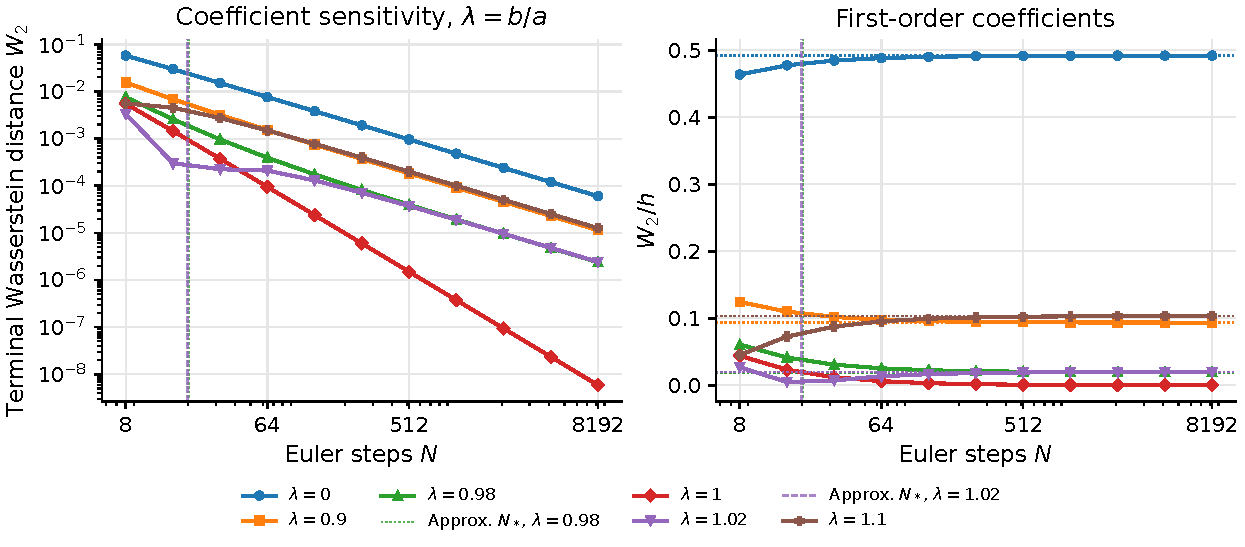
\includegraphics[width=\linewidth]{../results/figures/gaussian_sensitivity.pdf}
\caption{A fixed rotation mismatch gives first-order Euler distribution error for these Gaussian cases, with the parameters of Figure~\ref{fig:gaussian}. Each curve keeps $\lambda=b/a$ fixed as the grid is refined. The right panel shows error divided by $h$. For $\lambda\ne1$, this ratio tends to the positive value $|1-\lambda^2|c_0^{\rm G}$ shown by a horizontal dotted line. Section~\ref{sec:limits} defines $c_0^{\rm G}$. With matched rotation $\lambda=1$, the limit is zero. Vertical lines near $N=20$ estimate where the first- and second-order terms have similar size for $\lambda=0.98$ (dotted) and $1.02$ (dashed). Markers distinguish the error curves from their limits.}
\label{fig:sensitivity}
\end{figure}
\FloatBarrier

\subsection{Affine changes of coordinates, product distributions, and a dimension restriction}
\label{app:extensions}

A fixed affine change of coordinates can give distributions that are not radial in the original coordinates. For $\mathcal T(x)=d_{\rm aff}+Gx$ with $G$ invertible, set $\widetilde u(t,y)=Gu(t,G^{-1}(y-d_{\rm aff}))$ and $\widetilde p_t=\mathcal T_\#p_t$. Substitution into the differential equation and Euler update gives
\[
 \widetilde F_{s,t}\circ\mathcal T=\mathcal T\circ F_{s,t},\qquad
 \widetilde E_{t,h}\circ\mathcal T=\mathcal T\circ E_{t,h}.
\]
The transformed acceleration is $\widetilde{\acc}_t(\mathcal T(x))=G\acc_t(x)$. For every compact smooth test $\phi$,
\[
 \int\nabla\phi(y)\cdot\widetilde{\acc}_t(y)\,\widetilde p_t(\dd y)
 =\int\nabla(\phi\circ\mathcal T)(x)\cdot\acc_t(x)\,p_t(\dd x)=0.
\]
Because the affine map is invertible, $\phi\circ\mathcal T$ has compact support. The map also preserves the required smoothness, Lipschitz, growth, and moment assumptions, with different constants.

Write $s_{\min}(G)>0$ for the smallest singular value and $\|G\|_{\rm op}$ for the operator norm. Push forward any coupling to obtain the upper bound below, then apply that bound to $\mathcal T^{-1}$ to obtain the lower bound:
\[
 s_{\min}(G)W_2(\mu,\nu)
 \le W_2(\mathcal T_\#\mu,\mathcal T_\#\nu)
 \le\|G\|_{\rm op}W_2(\mu,\nu).
\]
Differences between particles from the same starting point satisfy the same norm bounds. These factors are fixed, so the positive limits in Theorem~\ref{thm:nonlinear} give orders $\Theta(h)$ and $\Theta(h^2)$ after the change of coordinates as well. The corrected distribution error is therefore smaller on sufficiently fine uniform grids. The estimates do not give exact coefficients or improvement on every grid. For example, $G=\operatorname{diag}(2,1)$ gives an elliptical mixture whose shape changes with time. This example is still an affine image of the symmetric one. Since $G(Du_0)G^{-1}$ need not be symmetric, the transformed base field need not minimize kinetic action.

We can also add independent stationary coordinates. This gives the product path $p_t\otimes\nu_{\rm stat}$ with field $(u_i,0)$, where $\nu_{\rm stat}$ has finite second moment. Projection onto the moving coordinates shows that the product $W_2$ is at least the original distance. Pairing each stationary coordinate with itself achieves this lower bound. Thus
\[
 W_2(\widehat p_k^i\otimes \nu_{\rm stat},p_{t_k}\otimes \nu_{\rm stat})
 =W_2(\widehat p_k^i,p_{t_k}).
\]
The stationary coordinates also leave particle error unchanged. Taking $\nu_{\rm stat}$ on $\R$ gives a three-dimensional example, and adding more coordinates gives examples in every dimension $d\ge2$. Independent products of moving planar examples also retain both error orders and strict improvement, since their squared $W_2$ distances add across components.

A dimension restriction applies if a tangent correction must cancel radial acceleration everywhere on a sphere while keeping the given radial coefficient. For $u(x)=\alpha(r)x+V(x)$ with $x\cdot V(x)=0$, differentiation in direction $V$ gives $x\cdot(DV)V=-\|V\|^2$. Differentiating the remaining acceleration terms yields
\[
 x\cdot\acc_u(x)=P(r)r^2-\|V(x)\|^2.
\]
Cancellation requires $\|V(x)\|^2=P(r)r^2>0$ at every point of each positive-radius sphere. In odd-dimensional space, such a sphere has even surface dimension, and the hairy-ball theorem requires every continuous tangent field to vanish somewhere~\citep[Theorem~2.28]{hatcher2002algebraic}. This rules out a tangent correction with the required cancellation at every point. Other fields can still have zero weighted divergence of acceleration, as the example with stationary coordinates shows.

\section{Robustness to an acceleration residual}
\label{app:robustness}

When only part of acceleration preserves the distribution, we shift the starting point along that part. The remaining acceleration contributes a first-order term to the global error bound. Proposition~\ref{prop:robustness} requires a bound on this remainder at every time, including Euler's evaluation times.

\begin{quote}
\textbf{Proposition~\ref{prop:robustness}, restated.}
Let $T>0$, $p_0\in\mathcal P_2$, and $p_t=(F_{0,t})_\#p_0$. Suppose $u$ is $C^2$ on a neighborhood of $[0,T]\times\R^d$, globally Lipschitz in space with constant $L$, and bounded at zero uniformly in time. Define $\acc$ and $\jerk$ as in Appendix~\ref{app:general}, and assume $C_j=\sup_t\|\jerk_t\|_{L^2(p_t)}<\infty$. Suppose
\[
 \acc_t=w_t+g_t,
 \qquad C_{w,2}=\sup_t\|w_t\|_{L^2(p_t)}<\infty,
 \qquad\sup_t\|g_t\|_{L^2(p_t)}\le\varepsilon.
\]
For each time, require $w_t\in C^1$ to be globally Lipschitz with a common constant $L_w$ and to have zero weighted divergence under $p_t$. With Euler's method and the grid defined above, put
$C_w=C_j/6+LC_{w,2}/2+TL_wC_{w,2}/8$. Then
\begin{equation}
 \max_k W_2(\widehat p_k,p_{t_k})
 \le e^{LT}\left(C_w\sum_jh_j^3+
                  \frac\varepsilon2\sum_jh_j^2\right)
 \le e^{LT}T\left(C_wH^2+\frac\varepsilon2H\right).
 \label{eq:robustness-full}
\end{equation}
\end{quote}
\begin{proof}[Proof of Proposition~\ref{prop:robustness}]
\label{proof:robustness}
For $X\sim p_t$, hold physical time fixed and follow the flow of $w_t$ for auxiliary duration $h^2/2$. This motion preserves $p_t$. The shift has $L^2$ norm at most $C_{w,2}h^2/2$ and remainder at most $L_wC_{w,2}h^4/8$ after its linear term. It supplies the $w_t$ part of the exact second-order displacement $h^2(w_t+g_t)/2$. The residual and exact-flow remainder stay in the error. The paired outputs therefore have root mean squared distance at most
\[
 \frac{C_j}{6}h^3+\frac{LC_{w,2}}{2}h^3+\frac{L_wC_{w,2}}{8}h^4
 +\frac\varepsilon2h^2.
\]
The Lipschitz estimate from the main proof bounds how much later Euler steps increase each error. Summing these contributions and using $\sum_jh_j^3\le TH^2$ and $\sum_jh_j^2\le TH$ proves the result.
\end{proof}

A time-dependent residual contributes $\frac12\sum_jh_j^2\varepsilon_{t_j}$. A bound on its time integral cannot control this sum, because the residual may be large at Euler's evaluation times. A small density-weighted divergence norm also need not give the required $L^2$ decomposition. Weighted $L^2$ projection separates acceleration into a part with zero weighted divergence and a remainder. This controls the norm, but it does not give the global Lipschitz bound required for the part that preserves the distribution.

The proposition bounds discretization error relative to the exact probability path of the approximate field. That path may differ from the intended path, so we must also estimate the error between the two paths. At the terminal time,
\[
 W_2(\widehat p_T^{\mathrm{approx}},p_T)
 \le W_2(\widehat p_T^{\mathrm{approx}},p_T^{\mathrm{approx}})
       +W_2(p_T^{\mathrm{approx}},p_T).
\]

\section{Dependence on the numerical solver}
\label{app:solver}

Euler and Heun require different rotations to cancel their leading Gaussian distribution errors. We first compare their expansions at a common step length, then pair two corrected Euler steps with one base-field Heun step to compare equal numbers of field evaluations.

\begin{proposition}[Euler and Heun for a fixed Gaussian rotation]
\label{prop:solver-dependence}
Let $T>0$, $a>0$, and let $\Sigma_0=C_0C_0^\top$ be positive definite in even dimension. Let $J^\top=-J$, $J^\top J=I$, $\Omega=C_0JC_0^{-1}$, $m_t=m_0+t\xi$, and $p_t=\mathcal N(m_t,e^{2at}\Sigma_0)$. For a fixed real $b$, use
\[
 v_b(t,x)=\xi+(aI+b\Omega)(x-m_t).
\]
On uniform grids with $h=T/N$, Euler satisfies
\begin{equation}
 W_2(\widehat p_N^{\mathrm E,b},p_T)
 =\sqrt{\tr\Sigma_0}e^{aT}\frac{T|a^2-b^2|}{2}h+O(h^2).
 \label{eq:gaussian-fixed-sensitivity}
\end{equation}
Define Heun by
\[
 x^*=x+hv_b(t,x),\qquad
 x^+=x+\frac h2[v_b(t,x)+v_b(t+h,x^*)].
\]
Its terminal error satisfies
\begin{equation}
 W_2(\widehat p_N^{\mathrm H,b},p_T)
 =\sqrt{\tr\Sigma_0}e^{aT}
       \frac{T|a(a^2-3b^2)|}{6}h^2+O(h^3).
 \label{eq:heun-leading-error}
\end{equation}
In particular, Heun's positive leading constant at $b=a$ is twice its constant at $b=0$. The leading Heun term cancels at $b=\pm a/\sqrt3$, giving an $O(h^3)$ bound in this family.
\end{proposition}

\paragraph{Proof idea.}
In centered whitened coordinates, each solver acts as a polynomial in $a+\mathrm i b$. The real part of the polynomial's logarithm gives the numerical log scale. We use this scale to calculate Gaussian distribution error.

\begin{proof}
The exact centered flow $e^{at}C_0e^{btJ}C_0^{-1}$ has the same covariance and mean for every $b$. Both solvers reproduce the affine mean exactly. For the centered whitened operator $B=aI+bJ$, Euler applies $I+hB$, while Heun applies $I+hB+h^2B^2/2$.

A matrix $cI+dJ$ multiplies whitened covariance by $c^2+d^2$, the squared complex modulus of $c+\mathrm i d$. Thus scalar complex calculations give the distribution error. With $w=h(a+\mathrm i b)$, the exact, Euler, and Heun scale factors are $e^{ah}$, $|1+w|$, and $|1+w+w^2/2|$. Writing $\Delta^{\mathrm{log}}$ for exact minus numerical log scale after $N$ steps, we use
\begin{align*}
 \log(1+w)&=w-\tfrac12w^2+O(w^3),\\
 \log(1+w+w^2/2)&=w-\tfrac16w^3+O(w^4).
\end{align*}
Taking real parts and multiplying by $N=T/h$ shows that
\[
 \Delta^{\mathrm{log}}_{\mathrm E}=\frac T2(a^2-b^2)h+O(h^2),\qquad
 \Delta^{\mathrm{log}}_{\mathrm H}=\frac T6a(a^2-3b^2)h^2+O(h^3).
\]
By the Gaussian scale identity,
$W_2=\sqrt{\tr\Sigma_0}e^{aT}|1-e^{-\Delta^{\mathrm{log}}}|$.
Substitution gives the stated errors. For Heun, the absolute cubic coefficients are $a^3/6$ at $b=0$ and $a^3/3$ at $b=a$, so Euler's correction doubles Heun's leading coefficient. The cubic coefficient instead vanishes at $b^2=a^2/3$.
\end{proof}

Euler's leading term cancels at $b=\pm a$, or only at $b=a$ if $b\ge0$ is required. For fixed $\delta_b$ with $b=a(1+\delta_b)$ and $b^2\ne a^2$, Eq.~\eqref{eq:gaussian-fixed-sensitivity} gives the positive first-order coefficient $\sqrt{\tr\Sigma_0}e^{aT}Ta^2|2\delta_b+\delta_b^2|/2$. Appendix~\ref{app:nonlinear-sensitivity} gives the corresponding result for nonlinear fields.

For this family, applying the matrix exponential of the full constant centered operator gives the exact solution. An exponential integrator that splits or approximates this operator needs a separate error analysis.

\begin{figure}[ht]
\centering
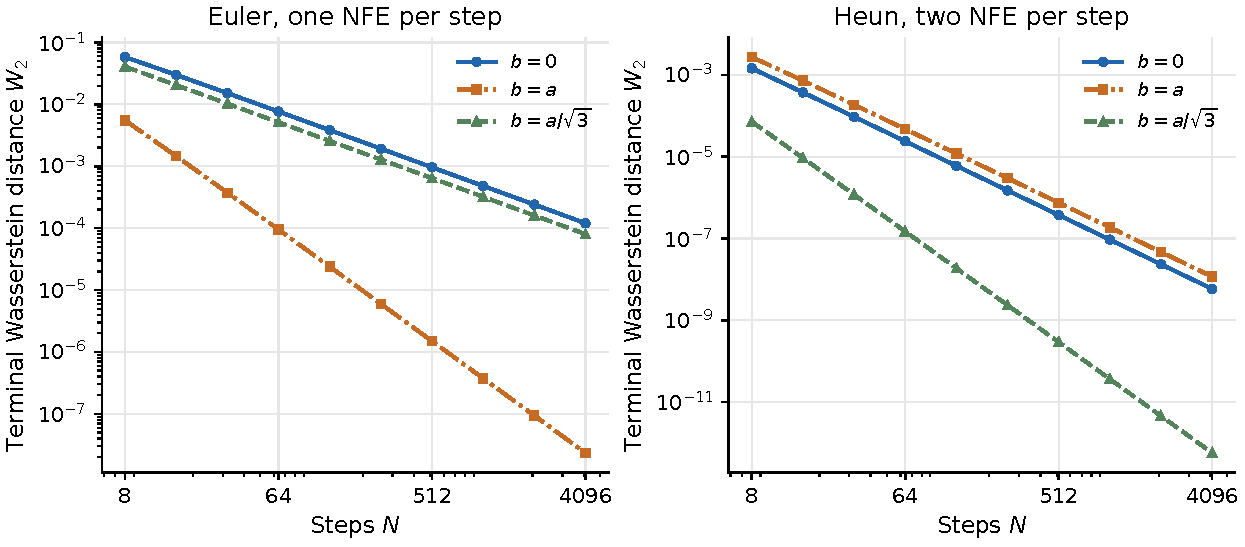
\includegraphics[width=\linewidth]{../results/figures/solver_dependence.pdf}
\caption{Euler and Heun require different rotations to cancel their leading distribution errors. Both methods use the Gaussian path and parameters of Figure~\ref{fig:gaussian}, with the same number of uniform steps. Rotation $b=a$ improves Euler but doubles Heun's leading coefficient relative to $b=0$. For Heun, $b=a/\sqrt3$ cancels the second-order term. Heun uses two evaluations per step, so the methods have unequal NFE here. Figure~\ref{fig:equal-evaluation}, Table~\ref{tab:few-evaluations}, and Table~\ref{tab:gaussian-higher-order} compare equal NFE.}
\label{fig:solver}
\end{figure}
\FloatBarrier

\subsection{Equal NFE for corrected Euler and base-field Heun}
\label{app:equal-evaluation}

\begin{proof}[Proof of Proposition~\ref{prop:equal-nfe}]
Let $N$ be even and $h=T/N$. In centered whitened coordinates, two corrected Euler steps of length $h$ have scale multiplier
\[
 \left(\sqrt{1+2ah+2a^2h^2}\right)^2
 =1+a(2h)+\tfrac12a^2(2h)^2.
\]
This is also the positive scale multiplier of one base-field Heun step of length $2h$. Both methods reproduce the affine mean. Their covariances match, so their Gaussian distributions are identical at every shared node. Euler uses one evaluation per step and Heun uses two, giving $N$ evaluations for each method on $[0,T]$. The same argument applies when consecutive Euler steps come in equal-length pairs on an otherwise nonuniform grid.
\end{proof}

\subsection{Corrected Heun and base-field RK3 at equal NFE}
\label{app:heun-rk3}

At $b=a/\sqrt3$, Heun's second-order distribution term cancels and the remaining third-order coefficient is positive. We calculate this coefficient and compare Heun with base-field RK3 using the same number of evaluations. Put $\zeta=a+\mathrm i b$, $R_2(w)=1+w+w^2/2$, and $C_\Sigma=\sqrt{\tr\Sigma_0}e^{aT}$. After $n=T/h$ uniform steps, Heun's errors are exactly
\begin{align}
 W_2^{\mathrm H,b}&=\sqrt{\tr\Sigma_0}\left|e^{aT}-|R_2(h\zeta)|^n\right|,\\
 e_{\mathrm p}^{\mathrm H,b}&=\sqrt{\tr\Sigma_0}\left|R_2(h\zeta)^n-e^{T\zeta}\right|.
 \label{eq:heun-exact-particle}
\end{align}
Here $e_{\mathrm p}$ is the root mean squared particle error from Section~\ref{sec:setup}. The formulas also apply to elliptical covariance, since a map difference $cI+dJ$ in transformed coordinates contributes covariance $(c^2+d^2)\Sigma_0$ in the original coordinates.

Since $\log R_2(w)=w-w^3/6+w^4/8+O(w^5)$, the choice $b=a/\sqrt3$ cancels the real cubic term. The remaining coefficients satisfy $\operatorname{Re}\zeta^4=-8a^4/9$ and $\operatorname{Im}\zeta^3=8a^3/(3\sqrt3)$. Thus
\begin{align}
 W_2^{\mathrm H,a/\sqrt3}&=C_\Sigma\frac{a^4T}{9}h^3+O(h^4),\\
 e_{\mathrm p}^{\mathrm H,a/\sqrt3}&=C_\Sigma\frac{4a^3T}{9\sqrt3}h^2+O(h^3).
 \label{eq:heun-attained-orders}
\end{align}
Both coefficients are positive, so distribution error is third order and particle error is second order.

For comparison, Kutta's three-stage, third-order Runge--Kutta method uses
\[
 k_1=v(t,x),\quad k_2=v(t+s/2,x+sk_1/2),\quad
 k_3=v(t+s,x-sk_1+2sk_2),\quad
 x^+=x+s(k_1+4k_2+k_3)/6.
\]
On the base field $v_0$, its centered scale factor is $R_3(as)=1+as+(as)^2/2+(as)^3/6$. Because $\log R_3(z)=z-z^4/24+O(z^5)$,
\[
 W_2^{\mathrm{RK3},0}=C_\Sigma\frac{a^4T}{24}s^3+O(s^4).
\]
The base-field Runge--Kutta map is a positive scalar dilation. Pairing particles from the same starting point is therefore optimal, so particle error equals distribution error.

For an evaluation count $N$ divisible by six, corrected Heun takes $N/2$ steps and base RK3 takes $N/3$. Substitution of $h=2T/N$ and $s=3T/N$ into the two error expansions proves
\[
 \lim_{N\to\infty}\frac{W_2^{\mathrm H,a/\sqrt3}}{W_2^{\mathrm{RK3},0}}=\frac{64}{81}.
\]
At the finite evaluation counts in Table~\ref{tab:gaussian-higher-order}, corrected Heun has 18.0--20.9\% smaller distribution error, while its particle error is larger.

\begin{table}[ht]
\centering
\begin{tabular}{rccc}
\toprule
NFE & \shortstack{Corrected field\\Heun $W_2$} & \shortstack{Base field, RK3\\$W_2$ and particle error} & \shortstack{Corrected field\\Heun particle error} \\
\midrule
12 & $1.677\times10^{-4}$ & $2.046\times10^{-4}$ & $3.904\times10^{-3}$ \\
48 & $2.790\times10^{-6}$ & $3.497\times10^{-6}$ & $2.581\times10^{-4}$ \\
192 & $4.426\times10^{-8}$ & $5.588\times10^{-8}$ & $1.636\times10^{-5}$ \\
384 & $5.547\times10^{-9}$ & $7.011\times10^{-9}$ & $4.100\times10^{-6}$ \\
\bottomrule
\end{tabular}

\caption{Corrected Heun has smaller distribution error but larger particle error than base-field RK3 at the listed evaluation counts. The parameters are those of Figure~\ref{fig:gaussian}, with $b=a/\sqrt3$ for Heun and $b=0$ for RK3. Both fields stay fixed as NFE increases.}
\label{tab:gaussian-higher-order}
\end{table}
\FloatBarrier

\section{Restrictions on the mean, second moment, and action}
\label{app:obstruction}

The acceleration condition requires the mean to move at constant velocity. It also determines kinetic action from the path's second moment. If a path fails these restrictions, no field in the stated class can satisfy the acceleration condition. Other ways to improve numerical accuracy may still be possible.

For Proposition~\ref{prop:obstruction}, let $X_t$ follow a global flow on $[0,T]$. Assume its trajectories and their first two derivatives are continuous, with $\dot X_t=u_t(X_t)$ and $\ddot X_t=\acc_t(X_t)$. One sufficient condition for the differentiations below is
\begin{equation}
 \E\sup_{0\le t\le T}
 [\|X_t\|^2+\|u_t(X_t)\|^2+\|\acc_t(X_t)\|^2]<\infty.
 \label{eq:moment-differentiation-assumption}
\end{equation}
More generally, require that the second moment can be differentiated twice under the expectation and that $u_t,\acc_t\in L^2(p_t)$. If $\acc_t$ has zero weighted divergence under the current distribution, then
\begin{equation}
 M''(t)=2\E\|u_t(X_t)\|^2,
 \qquad M(t)=\E\|X_t\|^2.
 \label{eq:moment-obstruction-full}
\end{equation}

\paragraph{Proof idea.}
The second derivative of the second moment contains kinetic energy and an acceleration term. To remove the acceleration term, we approximate squared distance by compactly supported tests and use zero weighted divergence. The remaining identity determines energy. This energy must be at least the infimum over fields satisfying the given continuity equation.

\begin{proof}[Proof of Proposition~\ref{prop:obstruction}]
Differentiating twice shows that
\[
 M''(t)=2\E\|u_t(X_t)\|^2+2\E[X_t\cdot\acc_t(X_t)].
\]
Condition~\eqref{eq:moment-differentiation-assumption} gives an integrable derivative bound, so dominated convergence and Cauchy--Schwarz justify differentiation under expectation. To test zero weighted divergence, replace squared distance by $\chi_n(x)\|x\|^2/2$, using the smooth compact cutoffs of Appendix~\ref{app:projection}. The gradient converges to $x$ in $L^2(p_t)$ as the second-moment tail vanishes. Since $\acc_t\in L^2(p_t)$, passage to the limit gives $\E[X_t\cdot\acc_t(X_t)]=0$ and proves Eq.~\eqref{eq:moment-obstruction-full}.

Let $K_{\min}(t)$ be the infimum of kinetic energy over fields satisfying the weak continuity equation for the path at time $t$. These competitors need not satisfy the acceleration condition. The chosen field has energy at least this infimum, giving $M''(t)\ge2K_{\min}(t)$. For a stationary distribution, $M''=0$ forces the field to vanish $p_t$-almost everywhere, or everywhere if the field is continuous and the density is positive throughout space.

For a centered radial dilation $p_t=(g(t)I)_\#p_0$, let $p_0$ be rotationally invariant and suppose $g>0$ is $C^2$ and $M_0=\int\|x\|^2p_0(\dd x)>0$ is finite. The base field is the gradient $v_t(x)=(g'/g)x$. The cutoff argument in Appendix~\ref{app:projection} places this gradient in the required closure. The projection identity then implies
\[
 K_{\min}(t)=M_0g'(t)^2,\qquad
 M''(t)=2M_0[g'(t)^2+g(t)g''(t)].
\]
When $g''(t)<0$, the necessary energy inequality fails. No field with the stated regularity and finite energy can then have zero weighted divergence of acceleration. For a scaling path that does admit such a field, its kinetic energy above that of the base field must equal $M_0g(t)g''(t)$.
\end{proof}

When $g''=0$, extra energy must be zero and the base acceleration is zero. If $g''>0$, an even-dimensional radial distribution can satisfy this necessary condition through
\[
 u(t,x)=\frac{g'}g x+b(t)Jx,\qquad b(t)^2=\frac{g''}g,
 \quad J^\top=-J,\quad J^\top J=I.
\]
Provided the square root has the required regularity, differentiation gives $\acc_u=[b'+2(g'/g)b]Jx$, which has zero weighted divergence for a radial distribution. Zeros of $g''$ require an additional check of square-root smoothness. Terminal accuracy can still occur when the local acceleration condition fails, through cancellation across steps (Appendix~\ref{app:local}).

\paragraph{Independent Gaussian interpolation at the midpoint.}
Independent interpolation pairs can have different kinetic energy from their conditional-mean field. For independent two-dimensional standard Gaussians $X_0,X_1$, let $X_t=(1-t)X_0+tX_1$. At $t=1/2$, the position depends on $X_0+X_1$, which is independent of $X_1-X_0$. The conditional mean velocity is therefore zero, although $\E\|X_1-X_0\|^2=4$. The path remains nonstationary, with variance decreasing before the midpoint and increasing afterwards.

\begin{proof}[Proof of Corollary~\ref{cor:mean-action}]
The same integrability assumption also lets us differentiate the mean twice under expectation. By Condition~\eqref{eq:moment-differentiation-assumption},
\[
 m'(t)=\E u_t(X_t),\qquad m''(t)=\E\acc_t(X_t).
\]
To evaluate the acceleration expectation, choose a smooth compact cutoff $\chi$ equal to one near the origin and put $\chi_n(x)=\chi(x/n)$. Testing Eq.~\eqref{eq:flux-null} with $\phi_n(x)=\chi_n(x)x_j$ gives gradients converging pointwise to $e_j$, with a bound independent of $n$. Since $\acc_t\in L^2(p_t)\subset L^1(p_t)$, dominated convergence gives $\E\acc_{t,j}(X_t)=0$. Hence $m''(t)=0$ and $m(t)=m(0)+t\E u_0(X_0)$.

Integrating Eq.~\eqref{eq:moment-obstruction-full} gives the action identity in Eq.~\eqref{eq:mean-action}. The moment assumption makes $M$ twice continuously differentiable, with endpoint derivatives taken from inside the interval. Thus the given path determines both the energy at each time and the total action for every field in this class.

If a gradient base field $v^\nabla$ generates the given path and satisfies the conditions in Section~\ref{sec:path-restrictions}, Eq.~\eqref{eq:projection} gives
\[
 \int_0^T\|u_t-v_t^\nabla\|_{L^2(p_t)}^2\dd t
 =\tfrac12\bigl[M'(T)-M'(0)\bigr]-\cA_T(v^\nabla).
\]
The path therefore determines the additional action within this class. The identity alone does not show that such a field exists.

The assumptions of Theorem~\ref{thm:distribution_order} also imply the required moment condition. With $U=\sup_t\|u(t,0)\|$, Gronwall's inequality gives
\[
 \sup_{0\le t\le T}\|X_t\|\le (\|X_0\|+TU)e^{LT}.
\]
Continuity gives $C_{a,0}=\sup_t\|\acc_t(0)\|<\infty$, and the common Lipschitz bounds give $\|u_t(X_t)\|\le U+L\|X_t\|$ and $\|\acc_t(X_t)\|\le C_{a,0}+L_a\|X_t\|$. Each squared time supremum is therefore bounded by $C(1+\|X_0\|^2)$ for finite $C$, which is integrable under the source second moment.
\end{proof}

\section{Minimum action among fields with the same path}
\label{app:projection}

We compare actions by using a gradient base field that can be approximated in mean square by compactly supported gradients. Such a field is orthogonal to every correction that preserves the probability path. For compactly supported potentials, zero weighted divergence gives this orthogonality directly. For the unbounded Gaussian and radial potentials, we use cutoff approximation to obtain the same result in mean square.

We use $\cV(p)$ for fields that are jointly continuous, have finite action, and are locally Lipschitz in space uniformly on compact time-space sets. Their flows must exist on $[0,T]$ and generate the given path. The action identity also holds for the larger class of finite-action fields satisfying the same weak continuity equation.

At each time, define the space of gradients and their mean square limits by
\[
 \mathcal G_t=\overline{\{\nabla\psi:\psi\in C_c^\infty(\mathbb R^d)\}}
 ^{L^2(p_t)}.
\]
Suppose $v_t\in\mathcal G_t$ for almost every time and $v$ has finite action. Let $r$ have finite action with $\nabla\!\cdot(p_tr_t)=0$ distributionally for almost every time. For every smooth compactly supported potential, $\mathbb E_{p_t}[r_t\cdot\nabla\psi]=0$. By continuity of the inner product in weighted $L^2(p_t)$, we also have $\mathbb E_{p_t}[r_t\cdot v_t]=0$. The cross term is therefore zero when we expand squared velocity and integrate, proving Eq.~\eqref{eq:projection}. Equal action requires $r=0$ almost everywhere under $dt\,p_t(dx)$, which means almost surely in position for almost every time. To obtain equality everywhere, we need the continuity and positivity argument below. Differences between fields satisfying the same continuity equation have the required zero weighted divergence. The existence of their particle flows is a separate requirement.

For the gradient fields used here, a finite second moment is enough to justify approximation by compactly supported gradients. Let $v_t(x)=\nabla\varphi_t(x)$, where
$\varphi_t$ has at most quadratic growth and its gradient has at most
linear growth, uniformly on the fixed time interval. Choose a smooth cutoff function
$\chi_n$ that is one on the radius-$n$ ball, zero outside the radius-$2n$
ball, and has $\|\nabla\chi_n\|\le C/n$. Then
\[
 \nabla(\chi_n\varphi_t)-\nabla\varphi_t
 =(\chi_n-1)\nabla\varphi_t+\varphi_t\nabla\chi_n.
\]
The squared approximation error is bounded by a constant times $\mathbb E_{p_t}[(1+\|X\|^2)\mathbf1_{\{\|X\|>n\}}]$, which vanishes by the finite second moment. For radial dilation, $\|X_t\|=g_t\|X_0\|$ with bounded $g_t$ gives one integrable tail bound for all times. The nonlinear path satisfies the same requirement through $\|X_t\|\le e^{(a+\eta)T}\|X_0\|$ in Eq.~\eqref{eq:radial-flow-growth}. Scaling and translating a fixed Gaussian gives the corresponding bound for the Gaussian path. Compactly supported gradients therefore converge in mean square both at each time and after time integration.

When every $p_t$ has positive density throughout space, equal action in $\cV(p)$ implies equality everywhere. A continuous difference nonzero at one point stays nonzero on an open time-space neighborhood. Every spatial ball in that neighborhood has positive $p_t$ mass, contradicting almost-everywhere equality under the path. The Gaussian path therefore has a unique minimizer in this continuous class.

\subsection{Gradient fields under the acceleration condition}
\label{app:gradient}
Under all assumptions of Theorem~\ref{thm:distribution_order}, suppose each $u_t$ is a gradient on $\R^d$. We prove that $\acc_t=0$ $p_t$-almost everywhere and that, for $p_0$-almost every start, Euler's method is exact on every finite increasing grid.

\begin{proof}[Proof of Proposition~\ref{prop:gradient-straight}]
\label{proof:gradient-straight}
A gradient velocity has a symmetric spatial Jacobian, so material acceleration is also a gradient. The growth bounds let us approximate acceleration by compactly supported gradients in the weighted norm. The acceleration condition makes acceleration orthogonal to all such gradients, so its norm must be zero.

Choose the normalized potential
$\psi(t,x)=\int_0^1 u(t,sx)\cdot x\dd s$.
Because $u_t$ is a gradient, $\nabla_x\psi=u_t$. The $C^2$ regularity of $u$ lets us differentiate in time and space. Symmetry of $D_xu_t$ then implies
\[
 \acc_t=\nabla q_{\rm acc,t},\qquad
 q_{\rm acc,t}=\partial_t\psi_t+\tfrac12\|\nabla\psi_t\|^2.
\]
Subtract $q_{\rm acc,t}(0)$ from this potential. With
$C_{a,0}=\sup_{t\in[0,T]}\|\acc_t(0)\|<\infty$, the common Lipschitz bound implies
\[
 |q_{\rm acc,t}(x)|\le C_{a,0}\|x\|+\tfrac12L_a\|x\|^2,
 \qquad \|\nabla q_{\rm acc,t}(x)\|\le C_{a,0}+L_a\|x\|.
\]
The growth bounds place $\acc_t$ in $\mathcal G_t$ by cutoff approximation. If the cutoff potentials are not smooth enough for the tests, convolution gives smooth compactly supported potentials whose gradients converge uniformly on a fixed compact set, hence in $L^2(p_t)$. Zero weighted divergence also makes $\acc_t$ orthogonal to $\mathcal G_t$, so
\[
 \|\acc_t\|_{L^2(p_t)}^2=0.
\]

At each fixed time, acceleration is zero almost everywhere. We need this conclusion along complete trajectories. Choose a countable dense set of times and intersect their full-probability sets of starting points. This intersection still has full probability. By continuity of $t\mapsto\acc_t(X_t)$, acceleration is zero at every time along each selected trajectory. Hence $X_t=X_0+t u_0(X_0)$ and $u_t(X_t)=u_0(X_0)$. Each Euler update from an exact point uses this constant velocity and reaches the next exact point. Euler is therefore exact on every finite increasing grid for the same set of starts.
\end{proof}

\section{Regular displacement interpolation}
\label{app:displacement}


Regular displacement interpolation moves each source point to its target at constant velocity along a straight line. Euler follows these trajectories exactly. Under the assumptions below, the field also minimizes action. \citet[Remark~7]{tao2026strain} note exactness on straight trajectories. The proposition gives sufficient assumptions on the map and proves exactness at successive grid points.

\begin{proposition}[Euler exactness on regular displacement interpolation]
\label{prop:displacement-euler}
Let $T>0$ and let $p_0$ be absolutely continuous with a finite second moment.
Let $\mathcal Q=\nabla\Phi_{\rm OT}:\mathbb R^d\to\mathbb R^d$, where
$\Phi_{\rm OT}\in C^2$, and suppose
\[
 0<\ell_- I\preceq D\mathcal Q(x)\preceq\ell_+ I
 \qquad\text{for all }x
\]
for fixed finite constants $\ell_-$ and $\ell_+$.
Define
\[
 \mathcal T_t(x)=(1-t/T)x+(t/T)\mathcal Q(x),\qquad
 p_t=(\mathcal T_t)_\#p_0,
\]
and define the field by
\[
 u(t,\mathcal T_t(x))=\frac{\mathcal Q(x)-x}{T}.
\]
The maps $\mathcal T_t$ are global diffeomorphisms, which means that they are continuously differentiable bijections with continuously differentiable inverses. The field is jointly continuous,
globally Lipschitz in space, and has linear growth. Its trajectories are
$X_t=\mathcal T_t(X_0)$.
On every finite increasing grid, Euler's method satisfies
\[
 \widehat X_k=\mathcal T_{t_k}(X_0)
\]
for every initial point. It is therefore exact for particles and their distributions at the grid points.

The map $\mathcal Q$ is the quadratic-cost optimal map from $p_0$ to
$p_T$. The displayed path is its displacement interpolation, and
\[
 \mathcal A_T(u)=\frac{W_2^2(p_0,p_T)}{T}.
\]
The field also minimizes action among finite-action fields satisfying this
fixed continuity equation, up to $dt\,p_t(dx)$-almost-everywhere equality.
\end{proposition}

\begin{proof}
The interpolating maps need global inverses to define the field at every position. With $s=t/T$, the symmetric derivative $D\mathcal T_t=(1-s)I+sD\mathcal Q$ has eigenvalues between $\min(1,\ell_-)$ and $\max(1,\ell_+)$. The lower bound gives strong monotonicity and injectivity, as well as properness, meaning that inverse images of compact sets are compact. The inverse function theorem makes the image open, while properness makes it closed. Since the image is nonempty and $\mathbb R^d$ is connected, the map is onto and has a global differentiable inverse. The uniform derivative bounds and field formula give the stated continuity, spatial Lipschitz continuity, and linear growth.

Each trajectory is affine in time. In particular,
\[
 \mathcal T_{t+h}(x)=\mathcal T_t(x)+h\frac{\mathcal Q(x)-x}{T}.
\]
If Euler reaches the exact point at $t_k$, its next evaluation gives the same constant particle velocity and its update reaches $\mathcal T_{t_{k+1}}(x)$. Induction proves exactness on every grid.

By the convex-gradient characterization, $\mathcal Q$ is the quadratic-cost optimal map~\citep[Section~6.2.3]{ambrosio2005gradient}. Each particle has constant velocity, giving action $\mathbb E\|\mathcal Q(X_0)-X_0\|^2/T$. Since the map is optimal, this action equals the stated Wasserstein formula.

For minimum action with the path fixed, it remains to place the velocity in the weighted gradient closure. At $y=\mathcal T_t(x)$, the spatial derivative is
\[
 D_yu(t,y)=\frac1T(D\mathcal Q(x)-I)
 \{(1-s)I+sD\mathcal Q(x)\}^{-1}.
\]
The matrices are symmetric and commute, so $D_yu$ is symmetric and $u_t$ is a gradient. Linear field growth gives at most quadratic potential growth, allowing cutoff approximation under finite second moments. If a cutoff potential is only $C^2$, convolution gives smooth potentials with uniformly convergent gradients on a compact support. Thus velocity lies in the weighted gradient closure, and the projection identity proves minimum action on the fixed path.
\end{proof}

These map assumptions are sufficient for both exactness and action minimization. Euler exactness alone needs only a well-defined field at evaluation times along constant-velocity straight paths. For a singular optimal-transport map, the existence of such a field needs a separate argument.

\section{A scaled rotated Gaussian coupling}
\label{app:fm}

We scale the rotated Gaussian pairing of \citet[Example~3.5]{liu2022marginal} to obtain the same probability path as independent Gaussian interpolation, using dependent endpoints. In even dimension, let $\sigma>0$, $J^\top=-J$, $J^\top J=I$, and $X_0\sim\mathcal N(0,I)$. With $\mathcal T_t=(1-t)I+\sigma tJ$ on $[0,1]$, each particle follows a straight line to a scaled rotation of its start. The endpoints are dependent, but $\mathcal T_t\mathcal T_t^\top=q_{\rm G}(t)I$ with $q_{\rm G}(t)=(1-t)^2+\sigma^2t^2>0$, giving the same Gaussian marginals as independent interpolation. The velocity field is
\begin{equation}
 u(t,x)=(\sigma J-I)\mathcal T_t^{-1}x
 =\frac{\sigma^2t-(1-t)}{q_{\rm G}(t)}x+\frac\sigma{q_{\rm G}(t)}Jx.
 \label{eq:fm-rotated-field}
\end{equation}
The radial term is the conditional-mean gradient velocity of independent Gaussian interpolation, while the rotation preserves each Gaussian marginal. Since $\mathcal T_{t+h}=\mathcal T_t+h(\sigma J-I)$, an Euler update from an exact point reaches the next exact point. Induction gives particle exactness on every grid, although rotation raises action above the gradient field by $d\sigma^2\int_0^1q_{\rm G}(t)^{-1}\dd t>0$.

For an anisotropic endpoint $CX_0$ with covariance $\Sigma_1=CC^\top$, this deterministic linear construction matches the independent-interpolation path exactly when $C+C^\top=0$. This follows by comparing the $t(1-t)$ covariance terms. An invertible real skew-symmetric matrix has two-dimensional blocks, so each eigenvalue of $CC^\top$ has even multiplicity. Conversely, equal eigenvalues can be paired into blocks $\sqrt\mu J$. The restriction applies only to this linear coupling class.

\section{Limits of action comparisons and evaluation schedules}
\label{app:schedules}

Our examples use fields with positive additional action. In a larger class of fields, the same numerical improvement can require arbitrarily little additional action. Euler uses the field only at its evaluation times, while action integrates squared velocity over time. A continuous correction can keep the same values at evaluation times and vanish outside short intervals around them.

For the Gaussian probability path in Appendix~\ref{app:fixed-gaussian}, fix a finite increasing grid and $a>0$. At step $j$, set
\[
 b_j=h_j^{-1}\sqrt{e^{2ah_j}-(1+ah_j)^2}.
\]
The inequality $e^{ah_j}>1+ah_j$ makes $b_j$ real and positive, with exact Euler covariance factor $(1+ah_j)^2+b_j^2h_j^2=e^{2ah_j}$. Set $b(t_j)=b_j$ at each evaluation time and extend these values by continuous functions supported in disjoint intervals of width at most $\delta$. Their sum $b_\delta$ is bounded and continuous, giving a global affine flow that preserves the Gaussian path. Shrinking the intervals keeps every Euler evaluation and output unchanged, while the added action satisfies
\[
 \tr(\Sigma_0)\int_0^T b_\delta(t)^2e^{2at}\dd t\longrightarrow0
 \quad\text{as }\delta\downarrow0.
\]
The grid is fixed and has finitely many evaluation times. The function heights are finite, so the action integral tends to zero as the total support length decreases. This gives the same numerical improvement with arbitrarily small additional action. The fields have no common bound on time derivatives.

\section{Numerical specification}
\label{app:numerics}

We calculate distances between full probability distributions, without using sample estimates. For the Gaussian examples, recursive matrix updates check the distance formulas and particle maps. For the nonlinear example, optimal radial transport gives the distances. We use independent reference calculations to check the nonlinear distances and their leading coefficients.

\subsection{Gaussian checks}

We evaluate the scalar Gaussian formulas at 80 decimal digits. We check the particle maps, covariances, and means against recursive Euler matrix updates in binary64 double precision. Each update starts from the preceding numerical result, with the mean moving at constant velocity. To calculate the Gaussian Wasserstein distance, we optimally align the covariance square roots by an orthogonal map. This avoids subtracting nearly equal trace terms. Quadrature along the exact flow gives an independent check of continuous action.

The nonuniform grid is $(0,0.04,0.17,0.43,0.72,1)$.

The Gaussian calculation uses $a=0.6$, $T=1$, and the fixed coefficients $b=0$ and $b=a$. In dimension two, the covariance is
\begin{equation}
 \Sigma_0=\begin{pmatrix}1.5&0.25\\0.25&0.75\end{pmatrix}.
 \label{eq:numerical-covariance}
\end{equation} Uniform step counts are the powers of two from one through 4096. Dimensions four and eight use $1,4,32$ uniform steps. All three dimensions also use the nonuniform grid above. For each higher dimension $d$, set $\Sigma_0=C_0C_0^\top$, where
\[
 (C_0)_{ii}=0.7+0.9\frac{i-1}{d-1},\qquad (C_0)_{i,i-1}=0.12\ (i\ge2),
\]
and all other entries vanish. For every dimension, the mean and drift components are
\[
 (m_0)_i=-0.4+\frac{i-1}{d-1},\qquad
 \xi_i=0.2-0.5\frac{i-1}{d-1}.
\]
The matrix $J$ uses consecutive two-dimensional quarter-turn blocks. We compare terminal squared distribution error, its maximum over grid points, and its sum over grid points. We also calculate error between particles from the same starting point and check the positive leading error coefficients in Appendix~\ref{app:fixed-gaussian}.

The contraction control uses $a=b=-0.6$, the stated two-dimensional covariance, and one step on $[0,1]$, with algebraic zeros recorded separately from floating-point residuals.

\subsection{Nonlinear example and reference calculations}

The nonlinear calculation uses $a=0.6$, $\eta=0.3$, $T=1$, and source $0.6\mathcal N(0,0.5^2I_2)+0.4\mathcal N(0,1.5^2I_2)$. The uniform step counts are powers of two from 8 through 4096. We also use the same unequal grid as above. For a spherical Gaussian component of scale $s$, $R_0^2/(2s^2)$ has density $e^{-z}$ on $z\ge0$. We therefore evaluate radius expectations by Gauss--Laguerre quadrature with 64, 128, or 256 nodes per component.

For the first reference calculation, we integrate log radius, angle, action, and the coefficient equations over time. We use SciPy 1.17.0's DOP853 ordinary differential equation solver, with primary relative and absolute tolerances $2\times10^{-13}$ and $2\times10^{-14}$. For an independent reference, we separate variables in the radius equation. With $r>0$, $a_+=a+\eta$, and $\ell=\log(R(T,r)/r)$, this gives the implicit equation
\[
 \frac\ell a-\frac\eta{2a a_+}
 \log\frac{a+a_+r^2e^{2\ell}}{a+a_+r^2}=T,
 \qquad aT\le\ell\le a_+T.
\]
This equation comes from integrating $1/f(r)$ between the source and terminal radii. Once we find the terminal radius, we integrate over radius to calculate angle, action, and leading coefficients. This calculation is independent of the time integration. Differentiating $\log f(R(s,r))$ gives $V(T,s;r)=f(R(T,r))/f(R(s,r))$ for $r>0$, so
\[
 \mathcal C_i(T,r)=f(R(T,r))\int_r^{R(T,r)}\frac{d_i(v)}{f(v)^2}\dd v.
\]
To separate quadrature error from reference error, we first increase the number of nodes with tolerances fixed. We then tighten the tolerances with the number of nodes fixed. The supplementary code includes all tolerances and comparison criteria.

We also compare independent particle updates in Cartesian and radius-angle coordinates, using source radii $(0.07,0.4,1,3,8)$ and angles $(0,0.3,1,2.1,4)$.

\subsection{Solver, sensitivity, and interpolation checks}

The solver calculations use $b=0$, $b=a$, and $b=a/\sqrt3$ on the same grids. We check the scalar stability factors against separate matrix updates. To study Euler's sensitivity, we use fixed ratios $b/a\in\{0,0.9,0.98,1,1.02,1.1\}$. The interpolation calculation uses $\sigma=1.5$. Its corrected field has zero error algebraically, and we record floating-point residuals separately. These computations check the numerical evaluation of the formulas. The proofs give the convergence orders and strict comparisons.


\subsection{Equal NFE}

For the nonlinear equal-NFE comparison, we keep the same source and coefficients and use $N\in\{2^j:j=1,\ldots,12\}$ evaluations. Euler takes $N$ uniform steps, while base-field Heun takes $N/2$. We calculate distances using 128 Gauss--Laguerre nodes per component and compare them with results from 64 and 256 nodes. All methods use the implicit exact-radius reference. We check this reference independently by time integration at relative tolerance $2.5\times10^{-14}$ and absolute tolerance $3\times10^{-15}$.

For base-field Heun, put $f(r)=\alpha(r)r$ and let $s=2T/N$. One radius step is
\[
 H_s(r)=r+\tfrac{s}{2}\{f(r)+f(r+sf(r))\}.
\]
Since $f'>0$, its derivative is
$1+\tfrac{s}{2}\{f'(r)+f'(r+sf(r))[1+sf'(r)]\}>0$.
The derivative is positive, so the radius map is increasing. The update also preserves angle. Pairing particles from the same starting point therefore matches angles and ordered radii. This pairing is optimal, so particle error equals $W_2$. We check all three methods with separate Cartesian updates. The smaller measured distribution error of corrected Euler applies to this source and these parameters.

Increasing quadrature from 128 to 256 nodes changes the errors by less than $1.8\times10^{-7}$ relatively, while the independent reference discrepancy is below $2.6\times10^{-8}$ of the corresponding numerical error.

The Gaussian Heun--RK3 comparison uses the parameters of Figure~\ref{fig:gaussian} at $12,48,192,384$ field evaluations. We evaluate the complex polynomials at 50 and 80 decimal digits and check them against independent matrix-stage recurrences at 70 and 100 digits. The extra precision controls error from subtracting nearby values in the distance calculation.

\subsection{Measured errors and refinement results}

Table~\ref{tab:nonlinear-results} gives the errors on the finest grid and order estimates $\log_2(e_{2048}/e_{4096})$, where $e_N$ is error after $N$ steps. We calculate the leading coefficients from independent radius integrals, without fitting the error curves. The primary calculation uses \NonlinearQuadratureOrder\ nodes per mixture component. Increasing this to 256 changes every reported terminal error, action, and coefficient by less than $8\times10^{-8}$ relatively. The largest reference discrepancy is below $3.2\times10^{-7}$ of the corresponding Euler error.

\begin{table}[!ht]
\centering
\caption{The nonlinear example has second-order corrected distribution error, although particle error remains first order. The calculation uses the source and parameters of Figure~\ref{fig:nonlinear}, 4,096 uniform steps, and \NonlinearQuadratureOrder\ quadrature nodes per mixture component. Observed order $\log_2(e_{2048}/e_{4096})$ measures the error reduction when the step count doubles, where $e_N$ is error after $N$ steps. The leading coefficients are limits of error divided by $h$, $h^2$, and $h$ in the three rows.}
\label{tab:nonlinear-results}
\begin{tabular}{lccc}
\toprule
Quantity & Error & Observed order & Leading coefficient\\
\midrule
Base distribution & $\NonlinearBaseFineError$ & $\NonlinearBaseOrder$ & $\NonlinearBaseCoefficient$\\
Corrected distribution & $\NonlinearCorrectedFineError$ & $\NonlinearCorrectedOrder$ & $\NonlinearCorrectedCoefficient$\\
Corrected particle & $\NonlinearParticleFineError$ & $\NonlinearParticleOrder$ & $\NonlinearParticleCoefficient$\\
\bottomrule
\end{tabular}
\end{table}

\FloatBarrier
The base and corrected actions are approximately $\NonlinearBaseAction$ and $\NonlinearCorrectedAction$. 

The Gaussian sensitivity calculation uses up to 8,192 steps to resolve the first-order limit for a 2\% coefficient mismatch. At this step count, all displayed scaled coefficients are within $0.5\%$ of their asymptotic predictions. We check the smallest Heun errors with independent matrix recurrences at 50 and 80 digits, including values below binary64 resolution. At 4,096 steps, the error ratio between $b=a$ and $b=0$ is $\HeunErrorRatio$, consistent with the limiting ratio two.






\FloatBarrier
